\documentclass[twocolumn,tighten]{aastex61}
\usepackage{hyperref}
\usepackage{pbox}

\AuthorCallLimit=500

\newcommand{\link}[1]{\href{#1}{\tt #1}}
\newcommand{\kms}{\,km~s$^{-1}$}
\def\squig{\sim\!\!}
\newcommand{\Msun}{\mbox{\,$M_{\odot}$}}
\newcommand{\Lsun}{\mbox{\,$L_{\odot}$}}

\newcommand{\graybox}[1]{\psboxit{box 0.7 setgray fill}{\spbox{#1}}}

\newcommand{\sinc}{\ensuremath{\mathrm{sinc}}}

\newcommand{\latin}[1]{{#1}}
\newcommand{\ie}{\latin{i.e.}}
\newcommand{\eg}{\latin{e.g.}}
\newcommand{\cf}{\latin{c.f.}}
\newcommand{\Sersic}{S\'ersic}
\newcommand{\vv}[1]{{\bf #1}}
\newcommand{\df}{\delta}
\newcommand{\dfft}{{\tilde{\delta}}}
\newcommand{\betaft}{{\tilde{\beta}}}
\newcommand{\erf}{{\mathrm{erf}}}
\newcommand{\erfc}{{\mathrm{erfc}}}
\newcommand{\Step}{{\mathrm{Step}}}
\newcommand{\ee}[1]{\times 10^{#1}}
\newcommand{\avg}[1]{{\langle{#1}\rangle}}
\newcommand{\Avg}[1]{{\left\langle{#1}\right\rangle}}
\def\simless{\mathbin{\lower 3pt\hbox
    {$\,\rlap{\raise 5pt\hbox{$\char'074$}}\mathchar"7218\,$}}} % < or of order
\def\simgreat{\mathbin{\lower 3pt\hbox
    {$\,\rlap{\raise 5pt\hbox{$\char'076$}}\mathchar"7218\,$}}} % > or of order
\newcommand{\iras}{{\sl IRAS\/}}
\newcommand{\petroratio}{{{\mathcal{R}}_P}}
\newcommand{\petroradius}{{{r}_P}}
\newcommand{\petronumber}{{{N}_P}}
\newcommand{\petroratiolim}{{{\mathcal{R}}_{P,\mathrm{lim}}}}
\newcommand{\band}[2]{\ensuremath{^{#1}\!{#2}}}
\newcommand{\Vmax}{\ensuremath{V_\mmax}}
\newcommand{\mmax}{\ensuremath{\mathrm{max}}}
\newcommand{\mmin}{\ensuremath{\mathrm{min}}}
\newcommand{\minmax}{\ensuremath{\mathrm{\left\{^{min}_{max}\right\}}}}
\newcommand{\fixMr}{\ensuremath{M_\fixr}}
\newcommand{\fixr}{\ensuremath{{r}}}
\newcommand{\fixredshift}{0.1}
\newcommand{\lya}{Ly$\alpha$}
\newcommand{\fixmag}[1]{\ensuremath{{^{\fixredshift}\!{#1}}}}
\newcommand{\fnl}{\ensuremath{f_{\rm NL}}}
\newcommand{\todo}[1]{{\bf TODO: #1}}
\newcommand{\Hband}{$H$-band}

% To-do:
%  * new Figure 1 with bigger labels

\setlength{\footnotesep}{9.6pt}

\newcounter{thefigs}
\newcommand{\fignum}{\arabic{thefigs}}

\newcounter{thetabs}
\newcommand{\tabnum}{\arabic{thetabs}}

\newcounter{address}

\shortauthors{Blanton {\it et al.} (2019)}
\shorttitle{Covariance-Regularized Reconstruction}

\begin{document}

\renewcommand{\arraystretch}{0.8}

\title{Covariance-Regularized Reconstruction of Images}

\correspondingauthor{Michael R.~Blanton}
\email{michael.blanton@gmail.com}
\author[0000-0003-1641-6222]{Michael R.~Blanton}
\affiliation{Center for Cosmology and Particle Physics, Department of Physics, New York University, 4 Washington Place, New York, NY 10003, USA}

\setcounter{address}{1}

\begin{abstract}
We discuss the problem of reconstructing an image from samples of its
values, and show how a method called covariance regularized
reconstruction (CRR) fits into a broader set of techniques addressing
this problem. Specifically, we address the estimation of values on a
rectangularly sampled grid based on a original set of irregular
samples, and we focus on astronomical applications. This problem has a
close mathematical relationship with deconvolution, image combination,
sinc-shifting, other interpolation tasks, as well as gravitational
lens reconstruction. We explain CRR, which we recently applied in the
context of image reconstruction but which is based on similar
techniques used in other contexts. We describe the relationship of CRR
to other methods. Its major advantages are that, to the greatest
extent possible, it retains the ``native'' spatial resolution of the
original sampling while yielding images whose pixel values have
uncorrelated errors. We describe the trade-offs between these
advantages and the advantages of more traditionally-regularized
deconvolution techniques. Finally, we show that for original samplings
that are already rectilinear, the CRR technique is identical to
techniques for shifting and combining samples already known under
certain conditions to conserve the information in the images (for
example, the sinc-shifting technique).
\end{abstract}

\section{Introduction}
\label{sec:intro}

This paper concerns the reconstruction of spatial or angular images
with uniform sampling, based on experimental data with nonuniform,
noisy sampling of varying spatial or angular
resolution. Reconstructions of this nature are often desirable either
for convenience or to consistently combine multiple data sets with
different samplings.  Here we concentrate on two-dimensional images
and astronomical applications, but the techniques described herein are
likely applicable in a broad range of circumstances.

We describe a method recently applied in this context called
covariance-regularized reconstruction, that provides reconstructions
whose individual pixel errors have low correlations with each other,
which can be shown in certain circumstances to contain the same
information content as the original samplings, and which appear to
degrade the intrinsic resolution of the sampling very little. The goal
of this paper is to compare this technique to other common methods and
describe the interrelationships of these methods.

Imagine that there is some function defining an image. This function
can be in any number of dimensions, but we will use the
two-dimensional case for the examples here.  Now imagine that the data
you have about this image is some sampling of its values at certain
locations. However this sampling has several properties, that are
common in situations involving real data:
\begin{itemize}
 \item The sampling isn't directly of the image, but of the image
   convolved with some resolution. So each sample is a projection of
   the image onto the ``kernel'' defining the resolution. The kernel
   may be different for each sample. 
\item The sampling is not on a rectilinear grid, and in fact may be of
  an arbitrarily irregular set of points.
\item The sampling is noisy, in the sense that the values you get from
  the sampling are the resolution-convolved image samples, plus some
  random noise term. We will assume that the noise is independent in
  each sample and that it is Gaussian.
\end{itemize}

This basic description applies to a number of different astronomical
data sets of interest. For example, shifting or rotating a normal
image from a charge-coupled device (CCD) can be described in this
fashion (though it doesn't necessarily need to be), as can the
combination (``stacking'') of multiple CCD images at different offset
positions or with significant astrometric distortions. Integral field
spectroscopy often produces image samples at each wavelength which are
not on a rectilinear grid, and which due to chromatic atmospheric
differential refraction are different for different
wavelengths. Gravitational lenses are a perhaps surprising example,
but the effect of the lens is only to change the kernel and the
location of the sampling; thus, our description also applies to
reconstructing source images behind gravitational lenses using a given
mass model (for example, see \citealt{warren03a, birrer15a}).

We should define the properties we would like our reconstruction to
have in an ideal case:
\begin{itemize}
\item It should be on a rectilinear grid.
\item It should minimally degrade the native resolution.
\item Fitting models to the reconstruction using the errors should be
  equivalent to fitting the original set of samples.
\item Errors in one pixel should have zero cross-correlation with
  errors in other pixels.
\end{itemize}
Importantly, our ideal case does not involve deconvolving the native
resolution and emphasizes retaining the simple statistical properties
for the errors (i.e. a diagonal covariance matrix). This emphasis is
related to the fact that many of the applications we have considered
can be low in signal-to-noise ratio; other definitions of ideal-ness
might be appropriate in other situations. This description (in
particular the last listed condition above) is equivalent to what
\citet{zackay17a} refer to as a ``proper'' image, and as we show in
the Appendix \ref{sec:zackay}, their method is equivalent to the CRR
method described here.

Section \ref{sec:model} describes a model problem, of irregular (also
called scattered) data samples with heterogeneous kernels. Section
\ref{sec:solutions} describes several classic approaches to this model
problem. Section \ref{sec:reconstruction} describes and tests our
method. Section \ref{sec:tests} tests all the methods on the model
problem against several benchmarks. Section \ref{sec:ifu} describes an
application to IFU data.  Section \ref{sec:lens} describes an
application to gravitational lens source modeling.  Section
\ref{sec:shift} describes an application to shifting or rotating
images and compares the method to classic sinc-kernel
shifting. Section \ref{sec:stack} describes an application to
coaddition of images and compares the method and results to other
methods.

\section{Model problem}
\label{sec:model}

The {\it anzatz} we adopt is that there exists some image we would
like to measure $R(x, y)$ where $x$ and $y$ represent some spatial or
angular coordinates (here taken to be in a two-dimensional space,
though the generalization to any other number of dimensions is
straightforward). We have experimentally sampled this image in various
locations which are arbitrarily well-known, the set of which can be
expressed as a vector of values $\vec{x}$ and $\vec{y}$, or $\{x_j\}$
and $\{y_j\}$. Each sample has some intrinsic spatial resolution we
refer to as a kernel $K_j(x, y)$; because of the experimental setup,
each sample $j$ is of the function $R(x, y)\otimes K_j(x,y)$. The
sampling produces a set of fluxes $\vec{f}$, or $\{f_j\}$. The
sampling is noisy with some standard deviation $\sigma_j$ for each
sample; each sample is statistically independent from the
others. Using this nonuniformly sampled data set $\vec{f}$ we want to
infer a set of flux values $\vec{S}$ (or $\{S_i\}$) at a uniform
rectilinear grid of pixel locations, which we will here refer to as a
reconstruction.

Astronomical data can have all of these properties, found separately
or together. First, a diffraction-limited telescope image has some a
resolution that sets the minimal kernel width, and in many
applications the atmosphere or the instrument provides an even broader
kernel. When combining multiple images, the kernel can vary due to
variations in the atmosphere or other effects. Some instruments, like
the Gaia satellite, have gross asymmetries in their kernel, and the
asymmetries are aligned differently with respect to the images for
different samples. Gravitational lenses can create very heterogeneous
kernels. Second, not all instruments have a rectilinear sampling
(particularly integral field spectroscopy), and even when they do,
multiple observations with the same instrument do not necessarily
align. Gravitational lenses also effectively provide an irregular
sampling of the source plane. Third, all of these observations have
intrinsic noise, and we want to be able to reliably interpret them
even in the noisy regime.

We will here define a specific model problem, where there are $M$
samples distributed between $-10 < x <10$ and $-10 < y < 10$. Each
sample has a kernel which is symmetric Gaussian with a standard
deviation chosen randomly, from a range we will choose differently in
different cases but which will generally be $\ge 1$. We will vary the
noise from case-to-case as well.  Figure \ref{fig:scattered-data}
shows an example data set of this variety.

The problem we want to solve is to produce a two-dimensional grid of
pixel values $\vec{S}$ that best represents (in the senses defined in
the introduction) the underlying image $R(x, y)$. We will use a grid
spacing of unity in our distance units, which will assure that our
pixel grid always at least Nyquist samples all kernel-convolved
images. We will place a central grid point at $(x, y) = (0, 0)$, and
use $n_x = n_y =21$, so the total number of grid points is $N=n_xn_y =
441$.

Before we begin, we make an observation about this model
problem. Imagine we have an explicit model $\vec{m}$ for the
observations whose parameters we desire to constrain. In that case,
because the noise is Gaussian, the likelihood for the model parameters
is $\mathcal{L} \propto \exp(-\chi^2/2)$, where
\begin{equation}
\label{eq:chi2}
  \chi^2 = \left(\vec{m} - \vec{f}\right)\cdot {\mathbf N}^{-1} \cdot
  \left(\vec{m} - \vec{f}\right),
\end{equation}
and $\mathbf{N}$ is the covariance matrix of the samples, which we in
this case is diagonal. If we manipulate the samples $\vec{f}$ in some
way---say, by resampling them onto a uniform grid---and fit the model
to the resampled data, we might in general change how $\chi^2$ depends
on the model parameters. However, if our resampling does not change
how $\chi^2$ depends on the model parameters, then it has retained
effectively the same information as the original set of samples.

% From scattered.ipynb
\begin{figure}[t!]
\centering
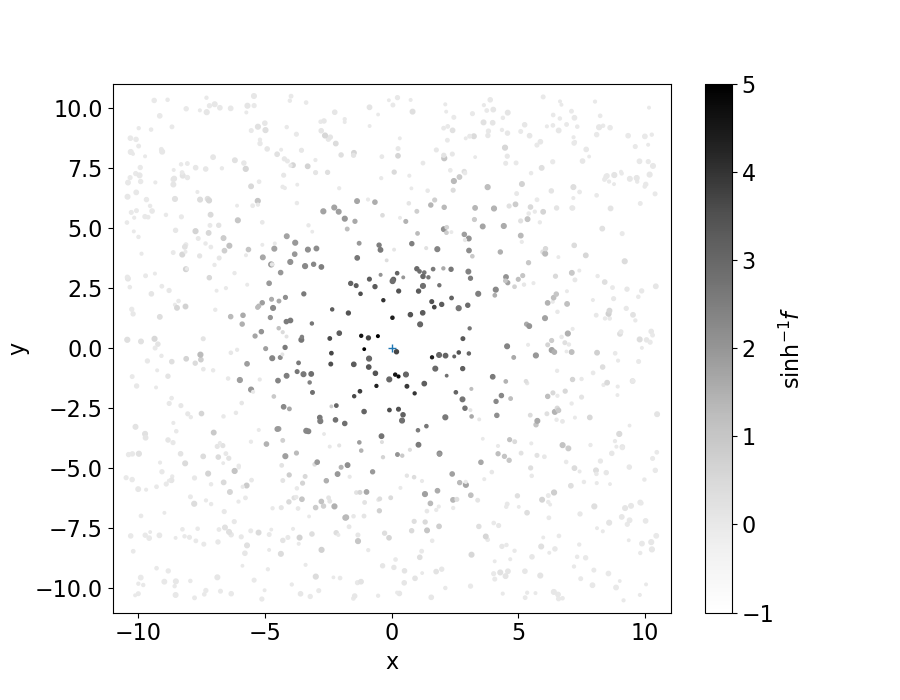
\includegraphics[width=0.49\textwidth, angle=0]{figures/scattered-data.png}
\caption{ \label{fig:scattered-data} Example of data in the model
  problem, for $M=1000$, with Gaussian standard deviations chosen
  randomly and uniformly between 1 and 4, and zero noise. Each point
  is a sample $f_j$, with a kernel width proportional to the point
  size, and the logarithm of the flux in the sample indicated by the
  color. The raw image is a point source at the center.}
\end{figure}

\section{Existing approaches to the problem}
\label{sec:solutions}

A number of methods exist to approach problems similar to that
described above. We will discuss these here in order to put the
motivation for our approach into context and to compare the
performance of our method with existing methods.

We divide the methods into two general categories. The first category
includes deconvolution methods, by which we mean here methods that
seek to infer the original image $R(x,y)$. We introduce these methods
because they help motivate our covariance-regularized reconstruction
method, but also to point out important features of deconvolutions
that affect whether we would choose to use them. We do not attempt a
complete review of deconvolution methods.

The second category we broadly term reconstruction methods. These
methods are harder to define in terms of their goals, but for a
uniform kernel $K$ most of them could be described as methods that
seek to infer $R(x,y)\otimes K(x,y)$. Covariance-regularized
reconstruction falls into this category.

\subsection{Deconvolution methods}
\label{subsec:deconvolution}

We introduce here some standard deconvolution methods. The goal of a
deconvolution method is to infer the ``undegraded'' image $R(x,y)$
based on the samples of $R(x,y)\otimes K_j(x,y)$. Typically, we seek
the values of $R(x,y)$ on a rectilinear grid in the
$x$--$y$ plane. If this deconvolution can be performed successfully
there are obvious advantages to it. However, there are disadvantages
as well that tend to be important in the presence of noise. First, in
the presence of noise it is always necessary to regularize the
deconvolution, and that regularization involves arbitrary choices that
render the estimate of $R(x,y)$ non-unique in ways that are hard to
characterize. Second, the different values of $R(x,y)$ on the grid
will inevitably have highly correlated errors, generally because
neighboring pixels can usually trade signal between each other while
still fitting the constraining data. Therefore, if noise is
significant relative to the signal, then fitting the deconvolution to
models requires tracking this covariance matrix. Standard
regularization methods do not mitigate this effect, and can worsen it.

\subsubsection{Unregularized and Tikhonov-regularized models}
\label{subsec:linear}

A straightforward way of approaching the model problem is to create a
nonparametric image designed explicitly to explain our sampled
fluxes. The idea is to determine a grid of pixel values $\vec{S}_F$,
representing the amplitudes of a set of delta functions, that explain
the sample values $\vec{f}$. 

Since each sample $j$ is the result of the convolution of the image
$R(x, y)$ with a kernel $K_j(x, y)$, the expectation value $\vec{m}$
for the flux samples of a model consisting of pixel values $\vec{S}_F$
can be written as a linear transformation:
\begin{equation}
\vec{m} = \mathbf{A}\cdot \vec{S}_F.
\end{equation}
Each column of $\mathbf{A}$ corresponds to a pixel in the
nonparametric image, and each row of $\mathbf{A}$ corresponds to an
observed sample; correspondingly, the values of the matrix are $A_{ji}
= K_j(x_i, y_i)$.  This model can perfectly reproduce any noise-free
set of observations $\vec{f}$ so long as the narrowest kernel
$K_j(x,y)$ is band-limited and is Nyquist sampled by the grid spacing;
this claim arises from the derivation of the Nyquist limit for
band-limited data.  To fit the parameters in the model image
$\vec{S}_F$ we minimize Equation \ref{eq:chi2} with this choice of
$\vec{m}$.

% from scattered-linear.ipynb
\begin{figure*}[t!]
\centering
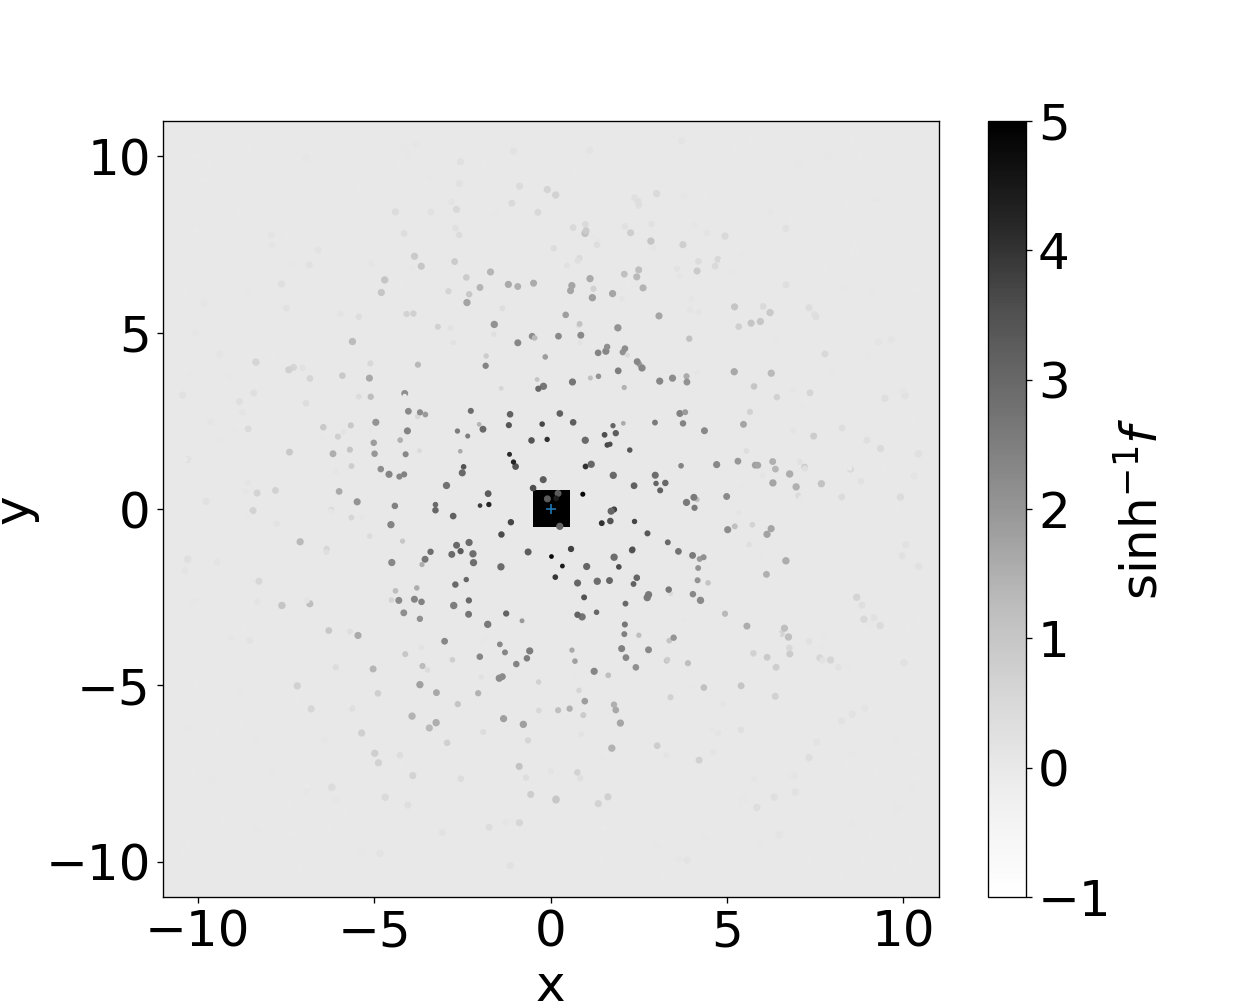
\includegraphics[width=0.32\textwidth, angle=0]
                {figures/scattered-unregularized-noiseless.png}
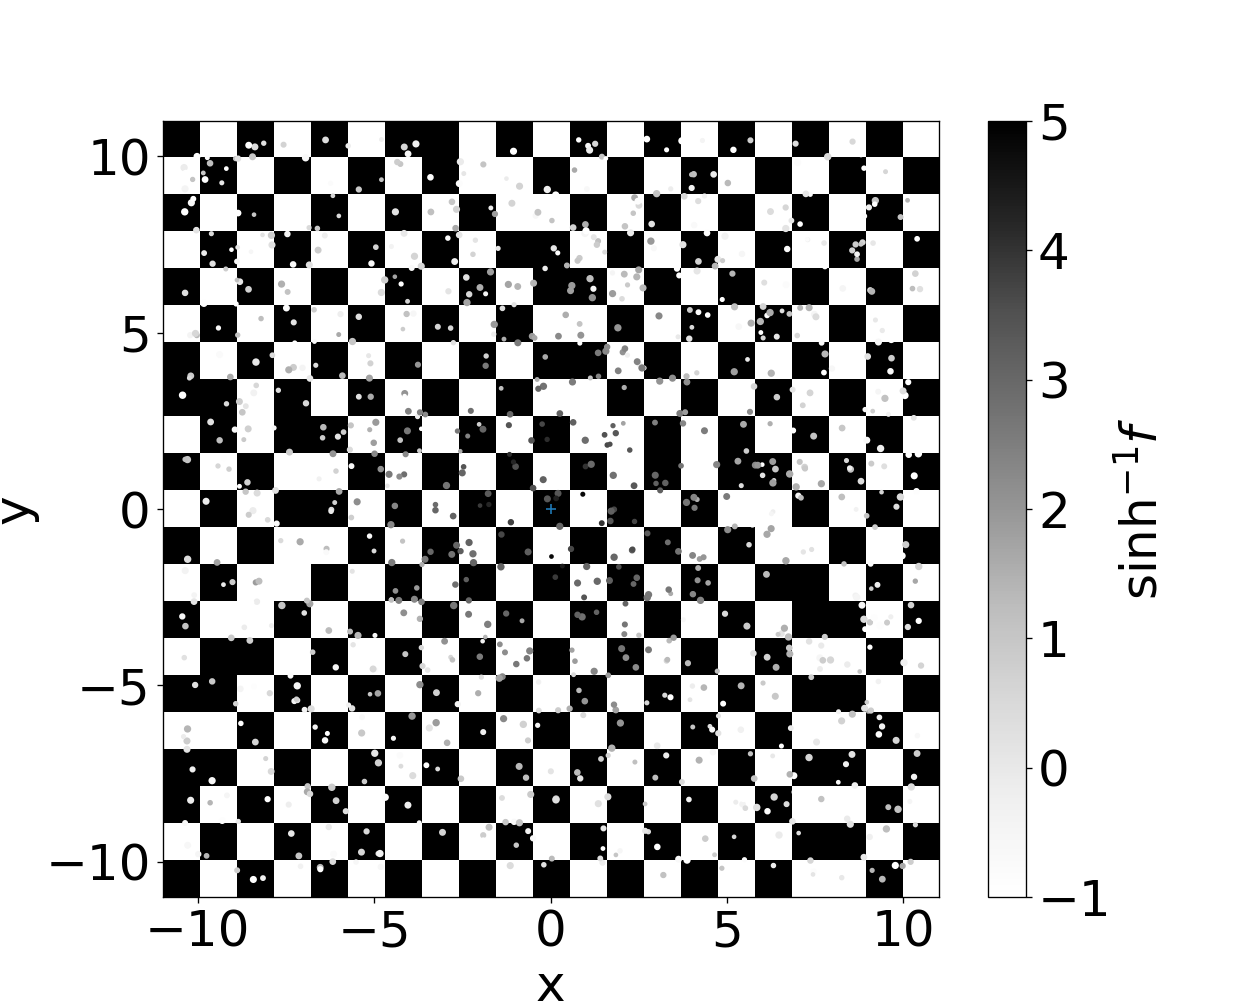
\includegraphics[width=0.32\textwidth, angle=0]
                {figures/scattered-unregularized-noisy.png}
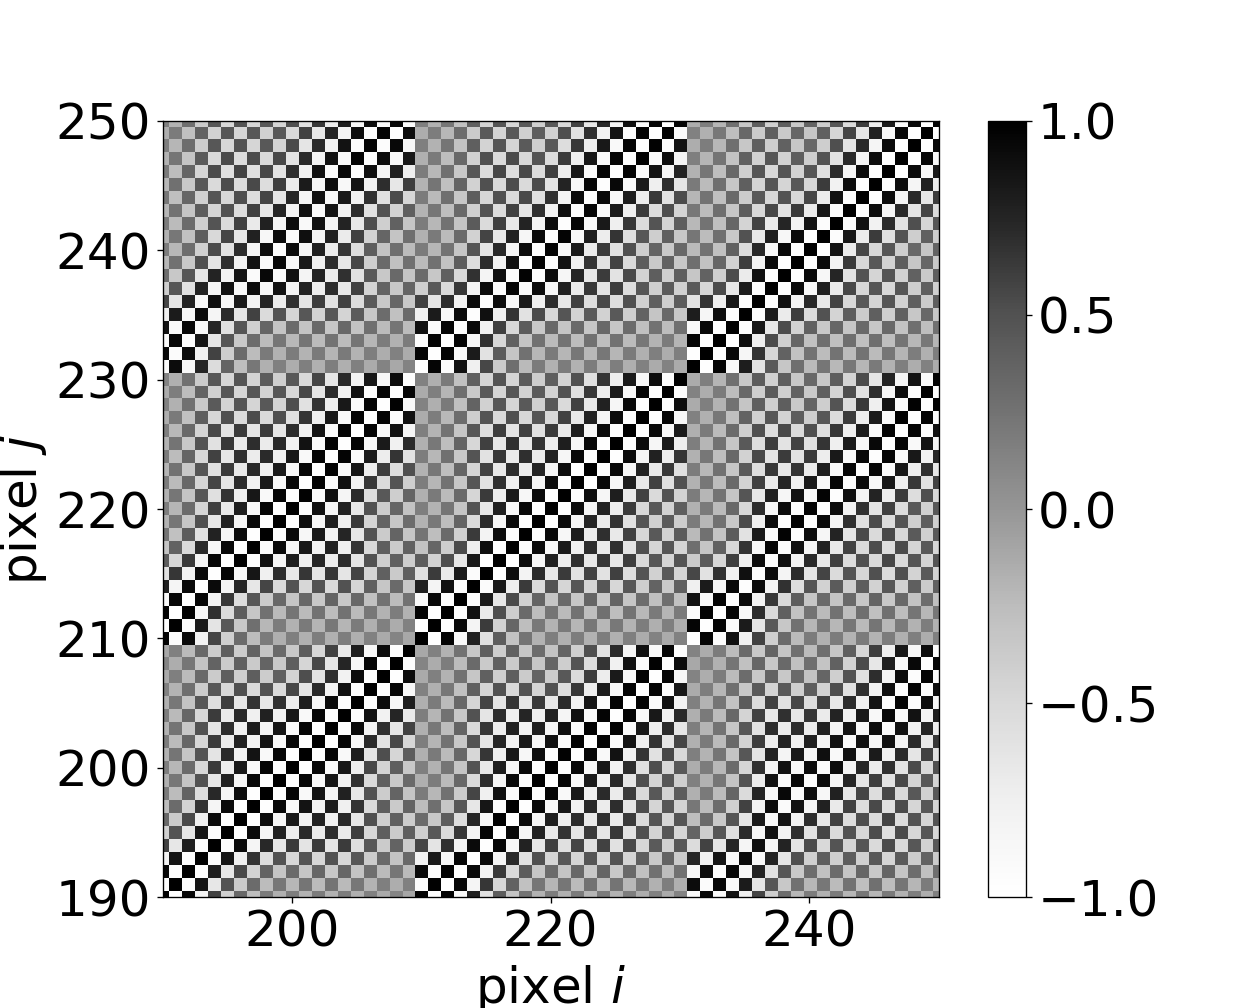
\includegraphics[width=0.32\textwidth, angle=0]
                {figures/scattered-unregularized-covar.png} \\
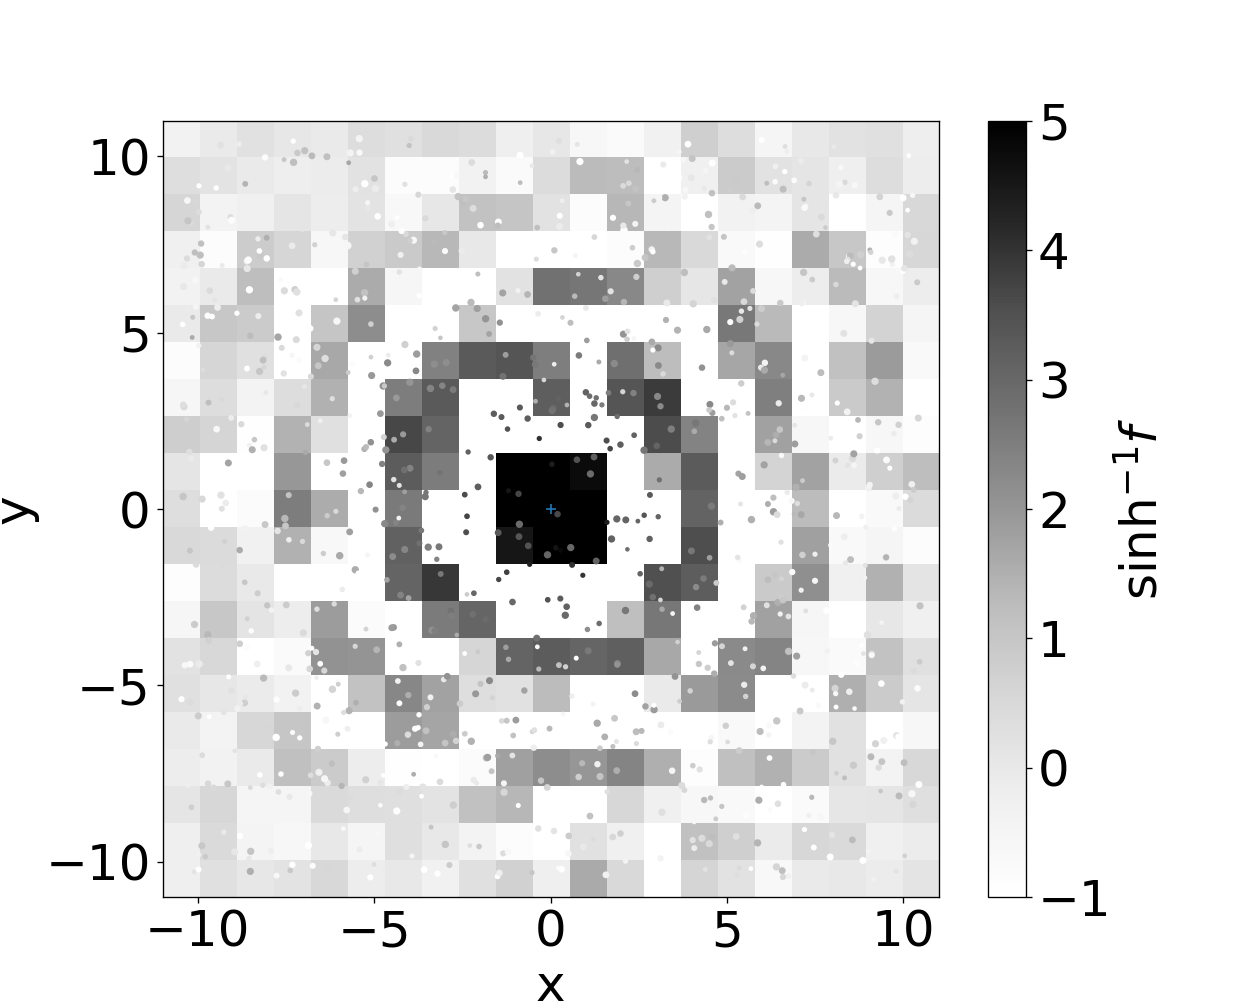
\includegraphics[width=0.32\textwidth, angle=0]
                {figures/scattered-regularized-T-noiseless.png}
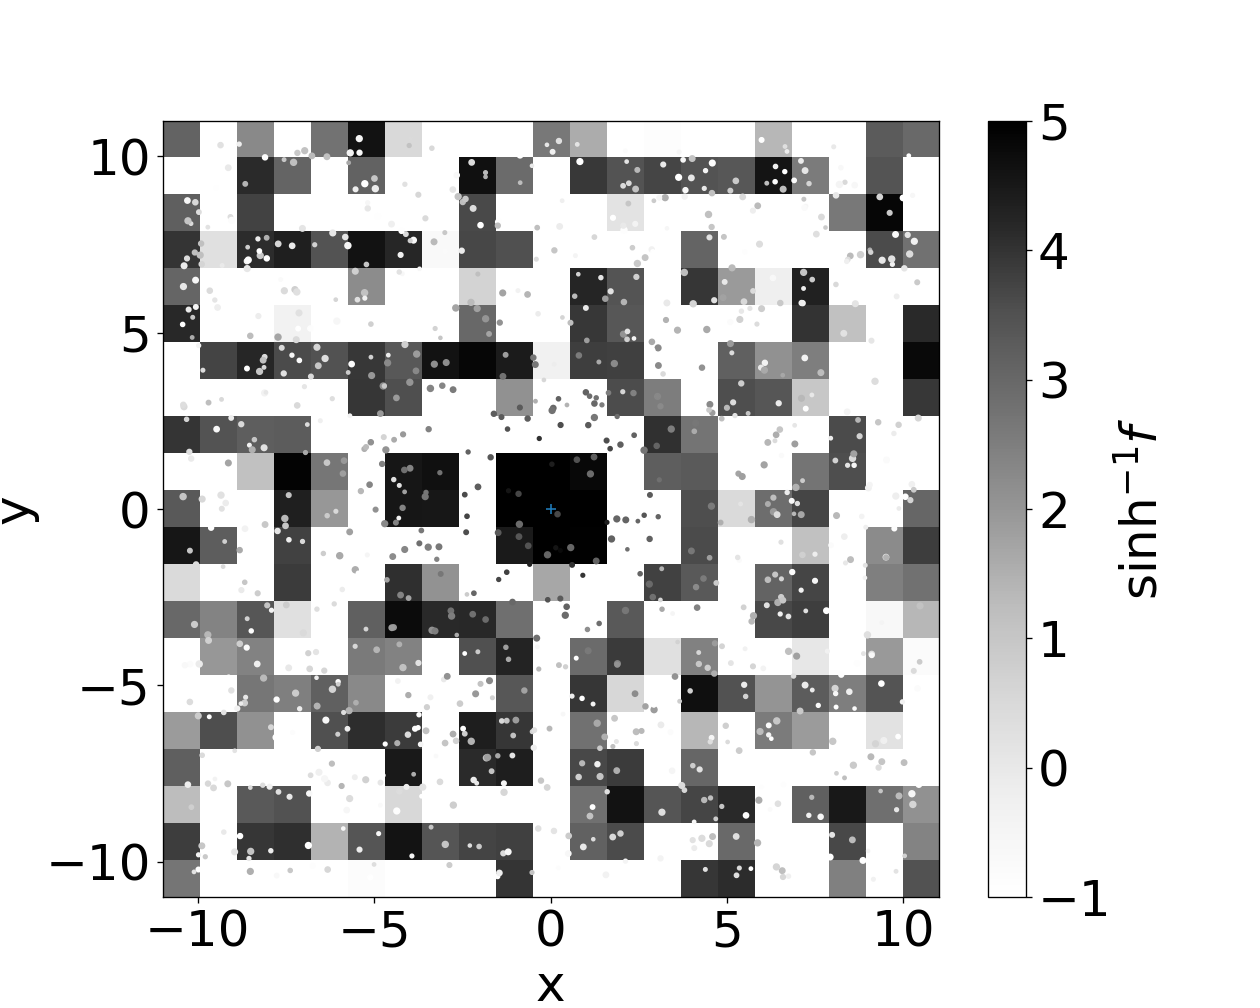
\includegraphics[width=0.32\textwidth, angle=0]
                {figures/scattered-regularized-T-noisy.png}
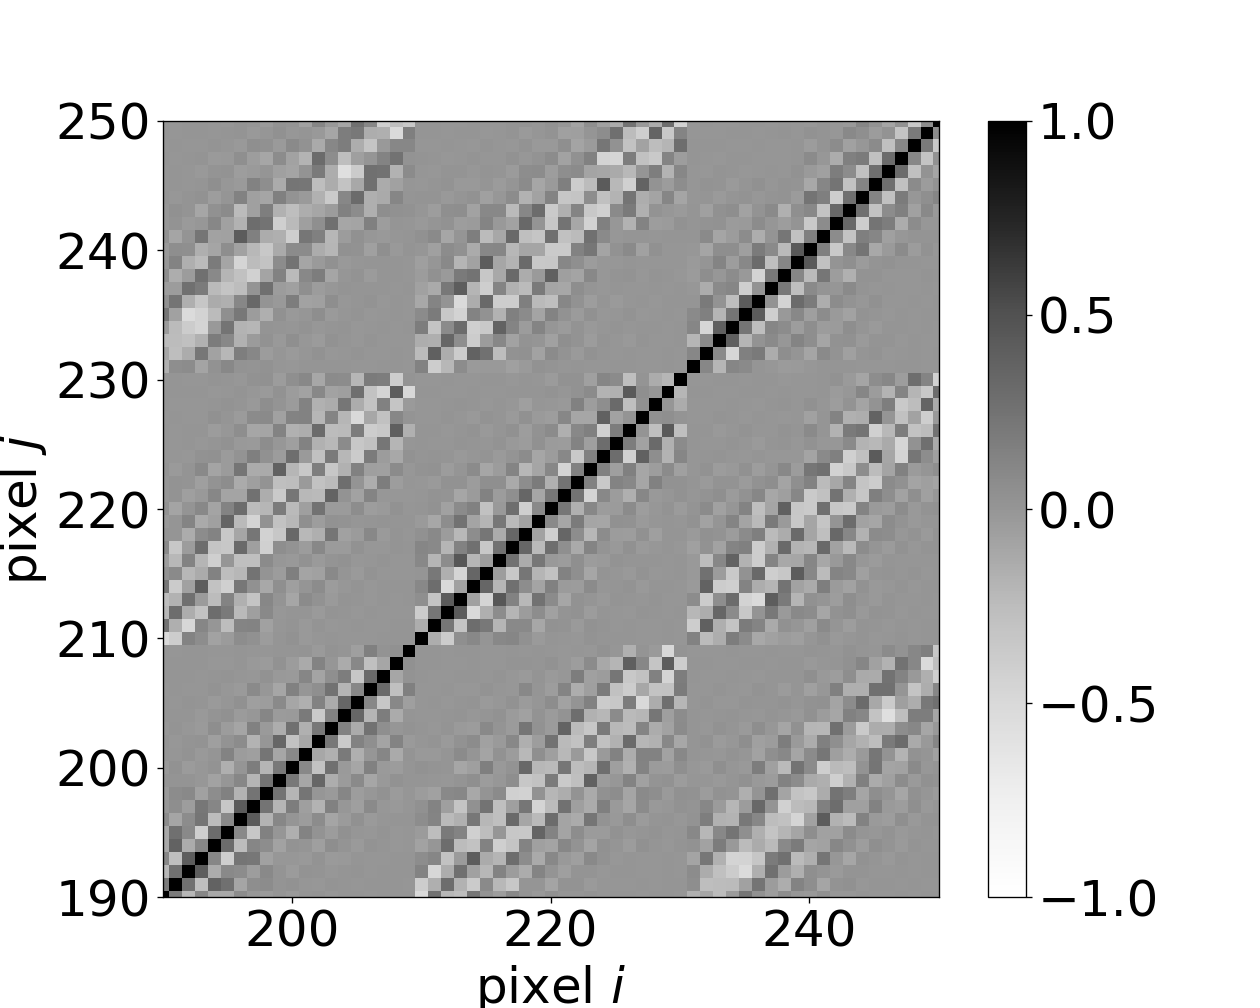
\includegraphics[width=0.32\textwidth, angle=0]
                {figures/scattered-regularized-T-covar.png}
\caption{ \label{fig:scattered-linear} Image reconstructions and
  correlation matrices using the methods of Section
  \ref{subsec:linear}. For each image reconstruction (left and middle
  columns), the dots show the function sampling locations and values,
  and the background image shows the reconstruction. Each panel uses
  the same set of sample locations and kernels, for a point source at
  the image center. The left column can be thought of as the PSF of
  the observations combined with the reconstruction method. For each
  method, we show a small section of the
  correlation matrix $C_{ij}/\sqrt{C_{ii} C_{jj}}$ near the diagonal
  (right columns).
  {\it Upper left:} Unregularized linear model applied to noiseless
  data. {\it Upper middle:} Unregularized linear model applied to data
  with noise per sample $10^{-3}$ of the total flux. {\it Upper
    right:} Correlation matrix for unregularized linear model fit,
  showing large off-diagonal terms. {\it Lower left:}
  Tikhonov-regularized linear model applied to noiseless data, with
  $\lambda=10^{-2}$.  {\it Lower middle:} Tikhonov-regularized linear
  model applied to noisy data, with $\lambda=10^{-2}$ and noise per
  sample $10^{-3}$ of the total flux.  {\it Lower right:} Correlation
  matrix for Tikhonov-regularized linear model.}
\end{figure*}

Since $\vec{m}$ is linear in the model parameters ($\vec{S}_F$), this
minization is quadratic and can be solved rapidly with matrix
inversion to find the values of $\vec{S}_F$ that minimize $\chi^2$.
For example, they can solved through the normal equations:
\begin{equation}
\vec{S}_F = \left(\mathbf{A}^T \cdot \mathbf{N}^{-1} \cdot
\mathbf{A}\right)^{-1}
\cdot \mathbf{A}^T \cdot \mathbf{N}^{-1} \cdot \vec{f}
\end{equation}
The covariance matrix $\mathbf{N}$ of the flux values $\vec{f}$ is
diagonal in the cases we consider in this paper. The covariance matrix
of $\vec{S}_F$ is given by:
\begin{equation}
\mathbf{C} = \left(\mathbf{A}^T \cdot \mathbf{N}^{-1} \cdot
\mathbf{A}\right)^{-1}
\end{equation}

We prefer here to use singular value decomposition (SVD) as follows:
\begin{equation}
  {\mathbf N}^{1/2} {\mathbf A} = {\mathbf U} \cdot \Sigma \cdot {\mathbf V}^T
\end{equation}
This decomposition is possible to achieve for any real matrices
$\mathbf{A}$ and $\mathbf{N}^{1/2}$ in terms of real $\mathbf{U}$,
$\mathbf{\Sigma}$, and $\mathbf{V}$, 
where $\mathbf{\Sigma}$ is diagonal, $\mathbf{V}$ is 
orthogonal ($\mathbf{V}\mathbf{V}^\mathrm{T} = \mathbf{1}$), and 
$\mathbf{U}$ is close to orthogonal
($\mathbf{U}\mathbf{U}^\mathrm{T}$ is diagonal with
ones for dimensions $i$ with $\Sigma_{i} \ne 0$
or zeros for dimensions $i$ with 
$\Sigma_i=0$).

That makes the inversion of the
problem easy so it is:
\begin{eqnarray}
\label{eq:sf}
  \vec{S}_F &=& {\mathbf V}\cdot\Sigma^{-1} \cdot {\mathbf U}^T \cdot
      {\mathbf N}^{-1/2} \cdot \vec{f} \cr
      &=& \mathbf{W}_F \cdot \vec{f}
\end{eqnarray}
In general, some values along the diagonal of $\Sigma$ may be zero or
very small (e.g. at double precision, of order $10^{-15}$ or so the
maximum value in $\Sigma$). When this occurs, the covariance matrix is
nearly or completely degenerate (non-invertible). In the inversion
above, we use the standard Moore-Penrose pseudo-inverse technique and
take $\Sigma_{ii}^{-1}=0$ if $\Sigma_{ii}=0$ (or very small). In
non-degenerate cases (when there is not a large dynamic range in
$\Sigma$) the result is identical to that found using the normal
equations; in degenerate cases, an infinite number of solutions exist
and the pseudo-inverse returns the solution that minimizes the norm
$|\vec{S}_F|^2$.

The upper left panel of Figure \ref{fig:scattered-linear} shows the
results of this method in the case there is no noise in the image. It
works essentially perfectly, as it should. This result shows how this
method works like a deconvolution---the kernel is fully deconvolved
out of the image model.

Under even a small amount of noise, however, this method is very
unstable. The upper middle panel of Figure \ref{fig:scattered-linear}
shows the results of adding noise per pixel at a level of $10^{-3}$ of
the total flux. A considerable amount of unnecessary noise is added;
in fact these effects appear even for much smaller amounts of
noise. 

We can understand the source of this effect by looking at the
covariance matrix of the results. The covariance matrix can be
written:
\begin{eqnarray}
\mathbf{C}_F &=& \mathbf{W}_F \cdot {\mathbf{N}} \cdot \mathbf{W}_F^T
\cr
&=&
\left(\mathbf{V}\cdot \mathbf{\Sigma} \cdot\mathbf{\Sigma} \cdot
\mathbf{V}^T\right)^{-1}
\end{eqnarray}
It is useful to look at the correlation matrix, which is defined
as:
\begin{equation}
\frac{C_{F,ij}}{\sqrt{C_{F,ii} C_{F,jj}}}.
\end{equation}
The upper right panel of Figure \ref{fig:scattered-linear} shows a
section of this correlation matrix. Clearly there are many strong
correlations among pixels.  It is clear that what is happening is that
neighboring pixels can generally cancel each other out in their
contribution to each sample, so they can become arbitrarily large in
the negative or positive direction, as long as their neighbors take
the opposite sign and cancel them out. This problem could be reduced
by taking larger pixels, but a much coarser grid would not sample the
kernel resolution well, which would reduce its ability to take best
advantage of the data.

A common method to control this sort of degeneracy is through a
regularization method. The simplest such method is Tikhonov
regularization, which modifies Equation \ref{eq:chi2} with the
addition of a term quadratic in the model parameters:
\begin{equation}
\label{eq:chi2_tikhonov}
  \chi^2 = \left(\vec{m} - \vec{f}\right)\cdot {\mathbf N}^{-1} \cdot
  \left(\vec{m} - \vec{f}\right) + \lambda^2
  \left|\Gamma\cdot\vec{S}_T\right|^2
\end{equation}
where in this case $\vec{m}= \mathbf{A}\cdot\vec{S}_T$ and $\vec{S}_T$
represents the Tikhonov-regularized result for some choice of $\Gamma$
and $\lambda$. An example of this usage can be found in
\citet{warren03a}. If $\Gamma$ is the identity matrix, this problem
can be reduced to a simple substitution of $\Sigma_{ii}^{-1}$ with
$\Sigma_{ii} / (\Sigma_{ii}^2 + \lambda^2)$ in Equation \ref{eq:sf}.

More complicated choices of $\Gamma$ lead to problems that are still
linear but that standard SVD does not conveniently decompose. However,
a generalized SVD (GSVD) exists that does so. For the two matrices
$\mathbf{N}^{-1/2} \cdot \mathbf{A}$ ($M\times N$) and
$\mathbf{\Gamma}$ ($N\times N$), a special case of GSVD is the
decomposition:
\begin{eqnarray}
\mathbf{N}^{-1/2}\cdot\mathbf{A} &=& \mathbf{U}\cdot \Sigma_1\cdot
\mathbf{R} \cdot \mathbf{Q}^T \mathrm{~and} \cr
\mathbf{\Gamma} &=& \mathbf{V}\cdot \Sigma_2\cdot
\mathbf{R} \cdot \mathbf{Q}^T,
\end{eqnarray}
where $\mathbf{Q}$ is $N\times N$ and orthogonal, $\mathbf{U}$ is
$M\times M$ and orthogonal, $\mathbf{R}$ is $N\times N$ and
non-singular, $\mathbf{V}$ is $N\times N$ and orthogonal, $\Sigma_1$
is $M\times N$ and diagonal, and $\Sigma_2$ is $N\times N$ and
diagonal. With this decomposition the solution becomes:
\begin{equation}
  \vec{S}_T = \mathbf{Q}\cdot\mathbf{R}^{-1}\cdot\left(
\Sigma_1^T\cdot\Sigma_1 + \lambda^2
\Sigma_2^2\right)^{-1} \cdot \Sigma_1^T \cdot \mathbf{U}^T
\cdot\vec{f}
\end{equation}
This approach is preferable to simply solving the normal equations for
Equation \ref{eq:chi2_tikhonov} because it requires only one
non-trivial inverse for many different choices of $\lambda$ and
because it allows the identification of the modes of the solution that
are affected by the regularization.

A simple but nontrivial choice for $\Gamma$ is designed to reduce the
differences between each pixel value and the average of its
neighbors. For this choice, each row of $\Gamma$ has $1$ in the
diagonal element and $-1/4$ in each element correponding to one of the
four closest pixels. The rows of $\Gamma$ corresponding to edge and
corner pixels instead have off-diagonal values of $-1/3$ and $-1/2$
respectively. 

The bottom left panel of Figure \ref{fig:scattered-linear} shows the
results of using this regularization under our model problem, with
$\lambda=10^{-2}$ and no noise in the data. This image can be thought
of as the PSF resulting from the combination of the image sampling and
the reconstruction technique.  This resulting PSF is narrow, but has
interesting ringing features whose origin is not obvious. Features
similar to these also occur for $\Gamma = \mathbf{I}$.  These features
become more pronounced, and different choices of $\Gamma$ yield more
dissimilar results, as $\lambda$ becomes larger.

The bottom middle panel of Figure \ref{fig:scattered-linear} reveal
the advantage of regularization when noise is added with an amplitude
per sample of $10^{-3}$ of the total flux. Unlike the unregularized
case, the general features of the noiseless image are maintained,
including the ringing features of the PSF. With our parameter choices
in this example, these ringing features are mostly subsumed into the
noise.

As the bottom right panel of Figure \ref{fig:scattered-linear} shows,
the noise itself exhibits correlations from pixel to pixel. These
correlations vary significantly depending on the exact relationship
between the sample locations, the sample kernels, and the pixel
locations, and can be both negative and positive. In our example, the
correlation coeffients are 0.15--0.20 out to separations of about
three pixels, and slowly decline after that; the typical pixel has
$\sim 40$ near neighbors with a correlation coefficient greater than
0.15. So in this example, fitting a model to the deconvolved data is
highly affected by these correlations if they are not properly
accounted for. Any time deconvolution is performed the impact of the
non-trivial correlation matrix needs to be evaluated to determine if
it is important to the problem at hand (which it may not always be).

In the Tikhonov regularization, $\lambda$ is a free parameter, as is
the detailed form of $\Gamma$.  Even very small $\lambda$ tends to
reduce the worst ``checkerboard'' features of the correlation matrix,
but neighboring pixels remain highly anticorrelated.  As $\lambda$ is
increased neighboring pixels transition from anticorrelated to
correlated and a broad positive correlation developed near the
diagonal of the correlation matrix. Meanwhile, as $\lambda$ increases
the PSF becomes broader and broader. The exact nature of the
dependence on regularization depends on a combination of the kernel
size and the reconstruction pixel scale, and must be carefully
evaluated for any deconvolution.

A key aspect of Figure \ref{fig:scattered-linear} is to recognize that
the PSF and the correlation matrix probe two different features of a
regularized deconvolution or any other sort of
reconstruction. Qualitatively, the PSF probes the coupling of the
signal in neighboring pixels, whereas the correlation matrix probes
the coupling of the noise in neighboring pixels. They both must be
known to characterize the relationship between a model for the
underlying image and the result obtained by the combination of our
instrument and our analysis.

\subsubsection{Linear models with nonnegative constraints}
\label{sec:nnls}

The linear deconvolution method can be adjusted by adding
regularization conditions that are not linear (i.e. are more complex
than the Tikhonov varity of methods). Nonnegative constraints are
tempting because we often expect the signal to be nonnegative, and yet
the degeneracies above arise in part from the fact that the solutions'
pixel values are allowed to be negative as well as positive.

Nonnegatively constrained deconvolution involves minimizing Equation
\ref{eq:chi2} under the conditions that $\vec{S}_F \ge 0$. Standard
techniques in quadratic programming exist that can readily solve the
linear problem under these constraints, at least at the scale of our
toy problem.  In the case of zero noise, the results are exactly the
same as the linear deconvolution method. That is, the method
successfully reconstructs a delta function source at the center.

\begin{figure*}[t!]
\centering
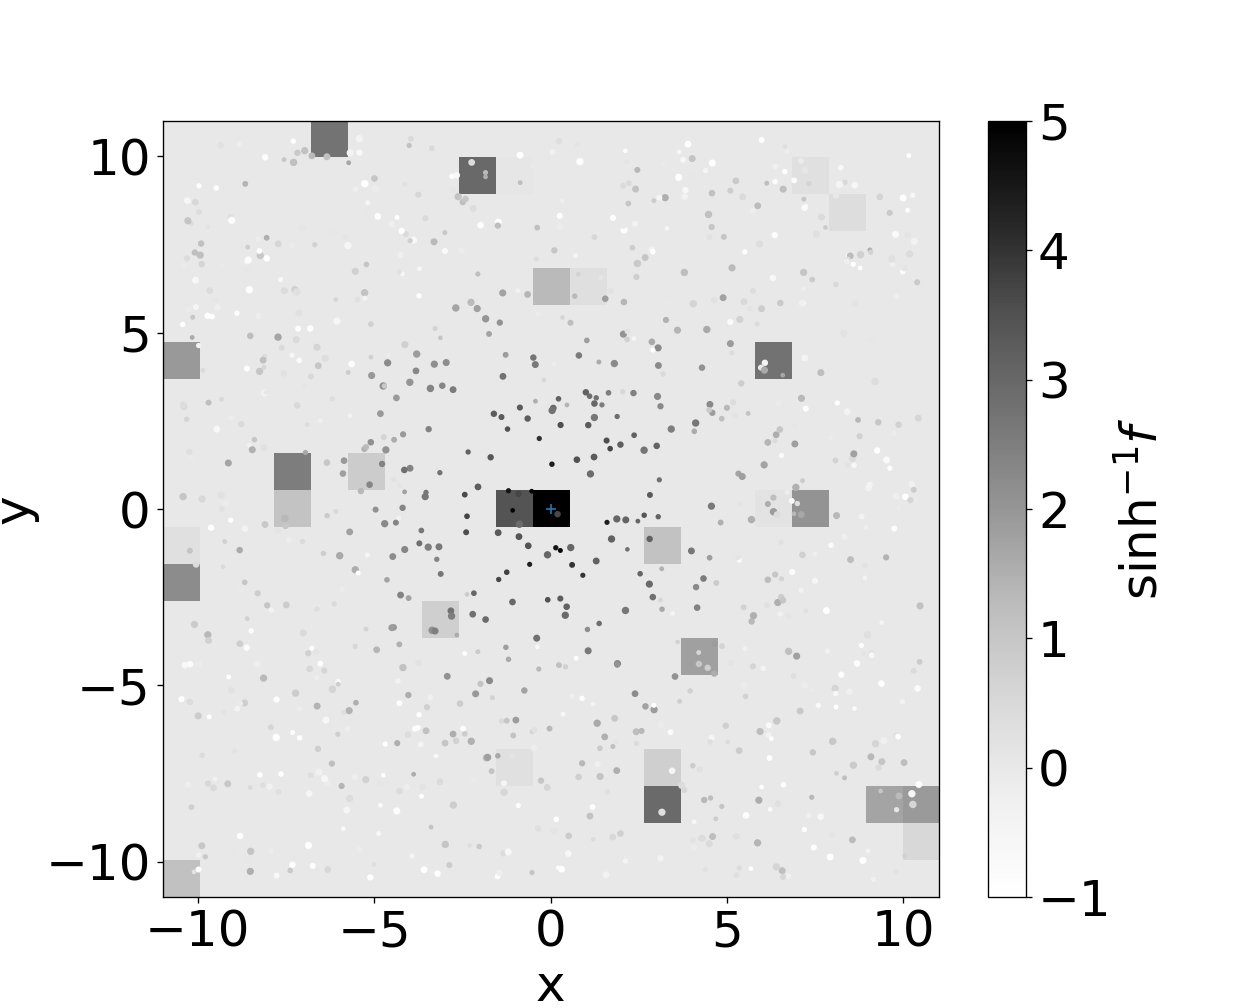
\includegraphics[width=0.24\textwidth, angle=0]
                {figures/scattered-nnls-noisy.png}
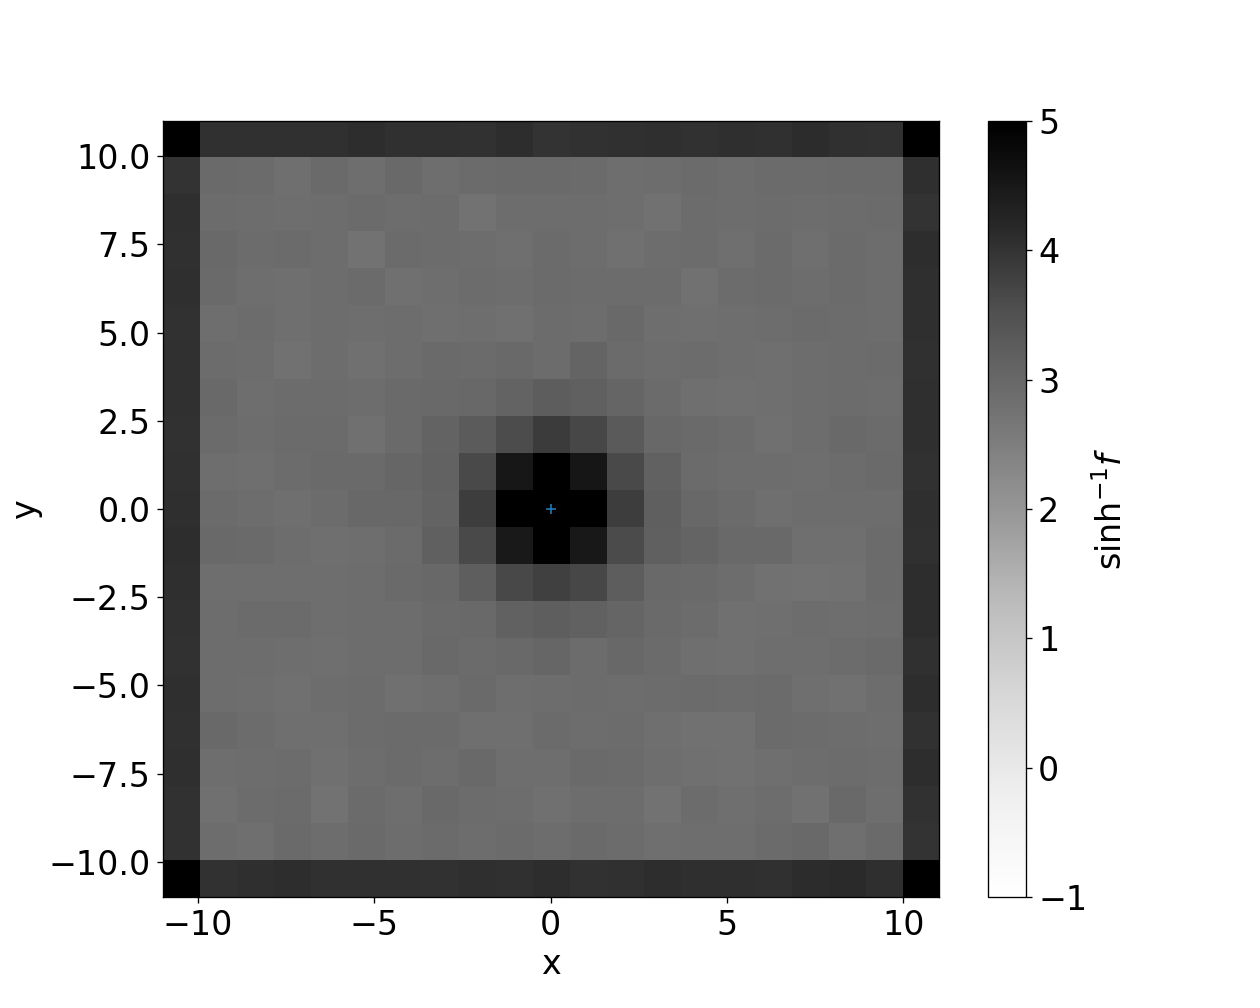
\includegraphics[width=0.24\textwidth, angle=0]
                {figures/scattered-nnls-mean-100.png}
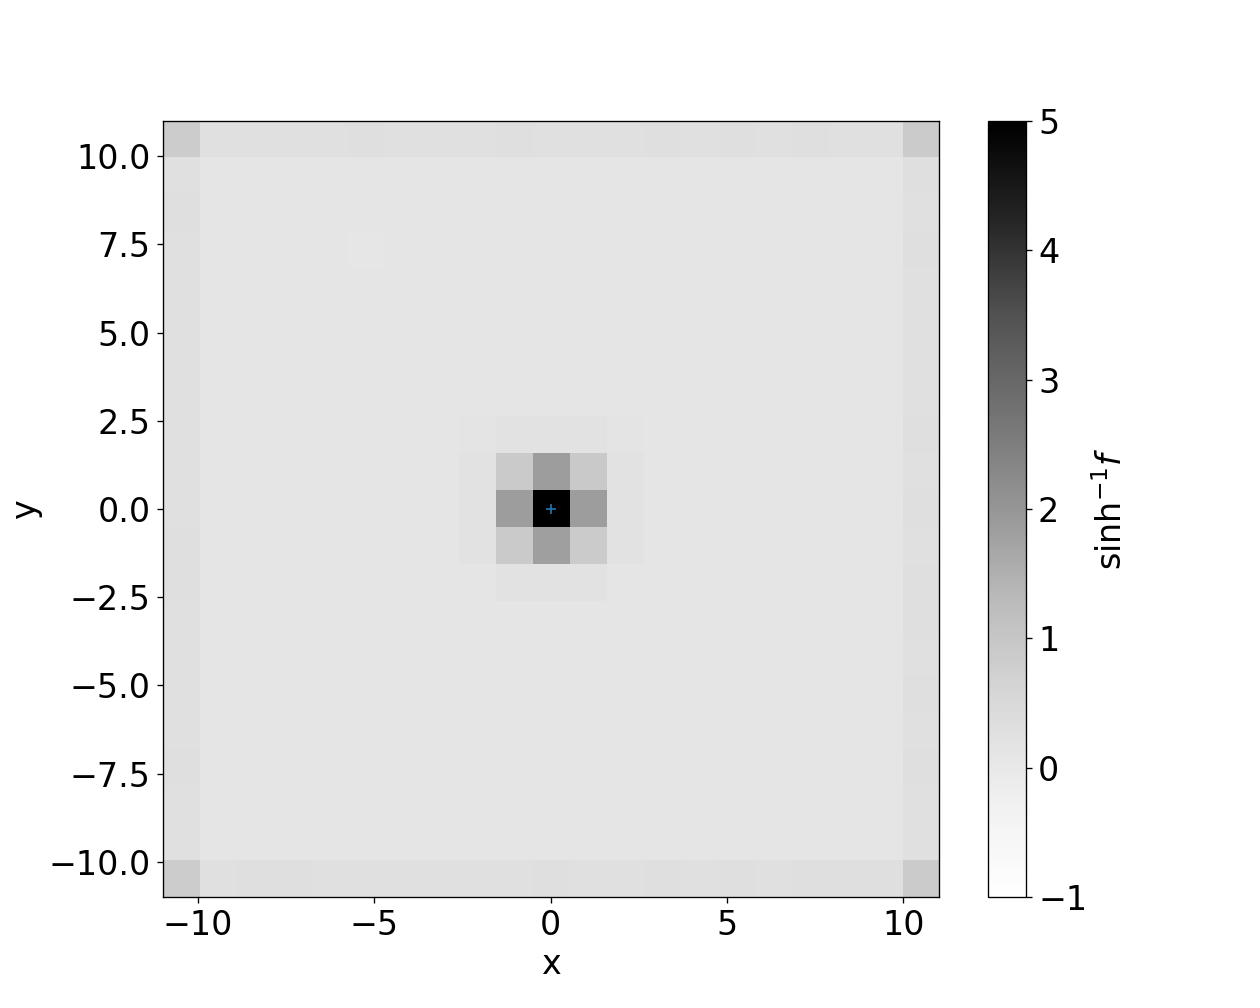
\includegraphics[width=0.24\textwidth, angle=0]
                {figures/scattered-nnls-mean-1.png}
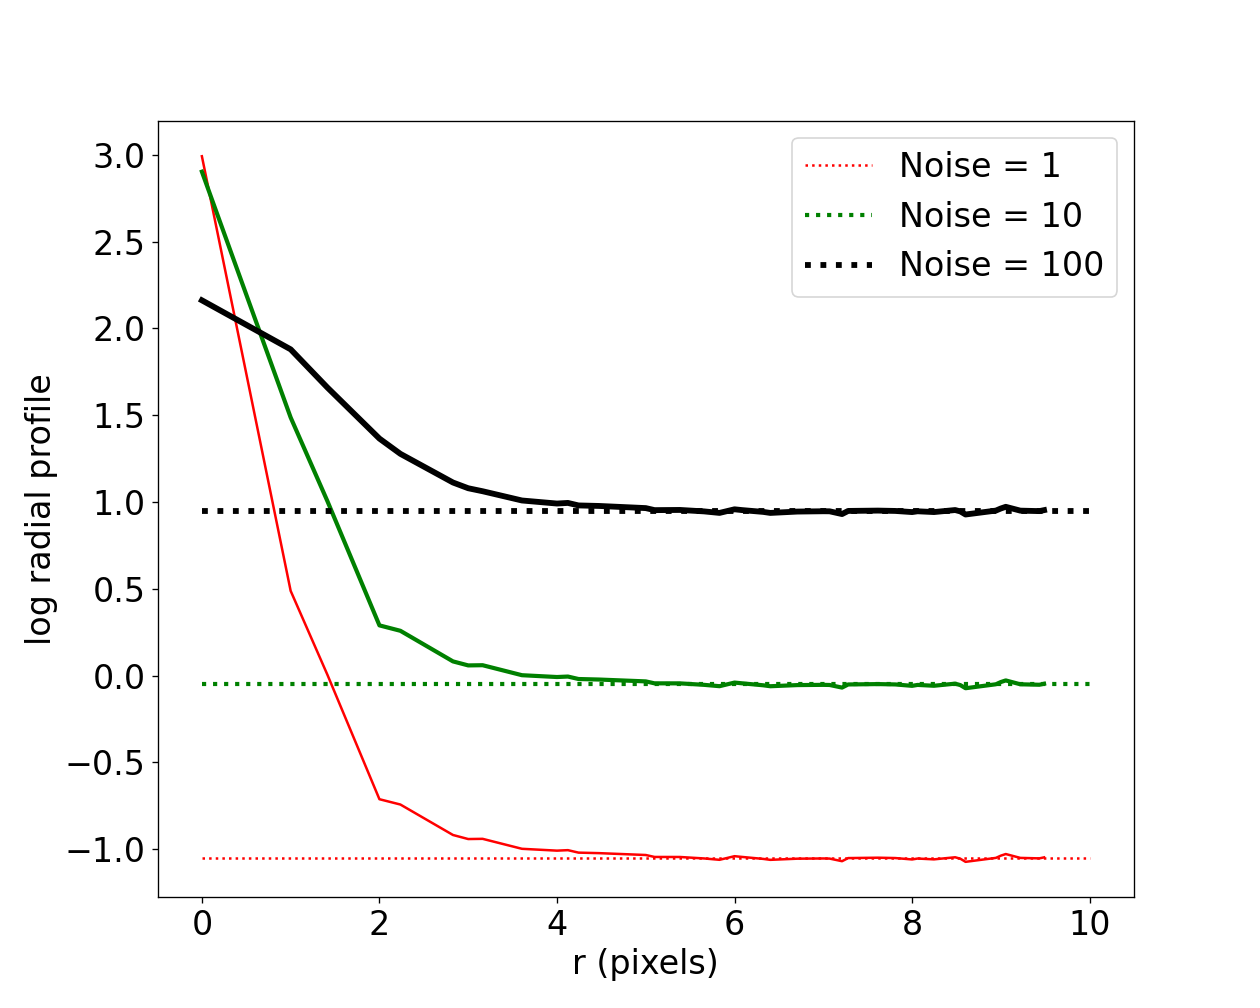
\includegraphics[width=0.24\textwidth, angle=0]
                {figures/scattered-nnls-mean-profile.png}
\caption{ \label{fig:scattered-nnls} Results for nonnegative least
  squares method applied to a point source input. {\it Left:} Single
  realization with noise per sample of $10^{-3}$ of the total
  flux. {\it Middle left:} Mean of 1000 realizations with noise per
  sample of $0.1$ of the total flux. {\it Middle right:} Mean of 1000
  realization with noise per sample of $10^{-3}$ of the total
  flux. {\it Right} Slice through mean of 25,000 realizations, for
  three noise levels (relative to a total flux of 1000), as labeled.}
\end{figure*} 

\begin{figure*}[t!]
\centering
%\includegraphics[width=0.24\textwidth, angle=0]
                %%{figures/scattered-nnls-flat.png}
%\includegraphics[width=0.24\textwidth, angle=0]
                %{figures/scattered-nnls-flat-covar.png}
%\includegraphics[width=0.24\textwidth, angle=0]
                %{figures/scattered-nnls-flat-dist.png}
%\includegraphics[width=0.24\textwidth, angle=0]
                %{figures/scattered-nnls-flat-dist-joint.png}
\caption{ \label{fig:scattered-nnls-flat} Results for nonnegative least
  squares method applied to a uniform signal distribution. {\it Left:}
  Single realization with noise per sample of $10^{-2}$ of the total
  flux. {\it Middle left:} Subsection of the covariance matrix based
  on 1000 Monte Carlo realizations. {\it Middle right:} Distribution
  of pixel values. {\it Right:} Joint distribution of pixel values of
  neighboring pixels; each point is a pair of pixels. For clarity near
  zero we have added a small amount of extra noise.}
\end{figure*} 

The effect of the nonnegative constraint becomes apparent in the
presence of noise.  Figure \ref{fig:scattered-nnls} shows the results
for a point source at the center with noise per sample of $10^{-3}$ of
the total flux. The left panel shows a single realization. This result
shows the power of the constraint; an extremely sharp image is
recovered without degeneracies appearing.

We can ask further what the mean response is to a point source, by
running 24,000 realizations. The middle left and middle right panels
show this mean response for two noise levels. The mean response is not
as narrow as each individual response, and the mean response appears
to depend on the signal-to-noise ratio. The far right panel shows the
radial profile of the mean response for three different noise levels
(passing through the location of the point source).

Two effects appear in Figure \ref{fig:scattered-nnls}.  First, a
background is evident, that becomes larger at higher noise
levels. This background is due to the fact that noise fluctuations
above zero lead to a response in the image but noise fluctuations
below zero lead to zero response. For Gaussian noise and a zero true
signal, the level of bias can be shown to be on average
$\sigma/\sqrt{2\pi N_{\rm eff}}$, where $N_{\rm eff}$ is the effective
number of samples contributing to each pixel. It must be that $N_{\rm
  eff} \propto \rho \sigma_g^2$, with $\rho$ being the density of
samples per pixel; for a constant $\sigma_g$ the constant of
proportionality is 4. The horizontal lines in Figure
\ref{fig:scattered-nnls} show this bias level estimated for the
simulation. For a non-zero true signal, the level of bias will be
less, but the bias is not possible to predict {\it a priori} because
the true signal is not known, which complicates statistical analysis
of the resulting image.

Second, the response becomes broader at higher noise levels, so that
the response is signal-to-noise ratio dependent. This nonlinearity is
a symptom of the nonlinearity of the method and a demonstration of the
fact that the mean response is not the PSF of the method.  For linear
methods the mean of the realizations would be the same as the
noiseless solution, because the linear operations of the method
commute with the mean. For nonlinear methods this commutation no
longer holds. Thus, there is no PSF, or in mathematical terms no
Green's function, that generally characterizes the response.

Another interesting case is the case of a uniform background within
the image area. This case characterizes how these deconvolutions will
work for more diffuse or extended sources. Unlike for linear methods,
the results for extended sources are not just a sum of the PSF
response, so we need to characterize them separately.  The left panel
of Figure \ref{fig:scattered-nnls-flat} shows the result of fitting
the results in the presence of noise per sample at about 1\% of the
background signal. For a diffuse background, the nonnegative
constraints still allow large fluctuations around that mean diffuse
value.

We can study these fluctuations with the covariance matrix, though as
we show below in this case the covariance matrix does not sufficiently
characterize the statistics of the noise. In this case, we need to use
a set of Monte Carlo realizations to determine the covariance matrix.
The middle left panel of Figure \ref{fig:scattered-nnls-flat} shows a
section near the diagonal of this covariance matrix estimated from
a 1000 realizations. There are strong negative off-diagonal values in
this covariance matrix, indicative of the degeneracies described
above.

The covariance matrix completely describes the distribution of a
multivariate Gaussian about its mean. However, the fluctuations in the
nonlinear case are far from Gaussian even when the input errors are
Gaussian. The middle right panel and right panels of Figure
\ref{fig:scattered-nnls-flat} demonstrate this non-Gaussianity, with
the probability distribution of pixel values and with the joint
distribution of these probabilities. There is a clear anticorrelation
of values when they are both non-zero, but in most cases one or the
other pixel of the pair is zero. A distribution like this one is not
fully characterized by a Gaussian and an analysis of this image that
accounted for the errors would not be correct if it assumed a Gaussian
distribution of errors.

The consequences of these properties are that characterizing the
resolution and noise of a nonlinear deconvolution, even the simplest
variety, can be complex. Typically, we do expect however that these
issues become less significant at higher signal-to-noise ratio.

We remark here briefly on the relationship between this method and
Richardson-Lucy deconvolution, which is commonly used in astronomy.
Richardson-Lucy maximizes the likelihood under a Poisson model for the
measured samples. The Poisson model is naturally nonnegative. Like
linear model with nonnegative constraints, it is a nonlinear method
and has very similar pitfalls. If the noise in the image is background
Poisson noise dominated (and the background is subtracted, not part of
the deconvolution), in fact Richard-Lucy decomposition reduces to the
nonnegative least squares technique.  Specifically, while its
performance can be reasonable for point sources, for extended
distributions it suffers from degeneracies that need to be
regularized. The Richardson-Lucy method is iterative, and a common
regularization is to provide a stopping condition before convergence;
this regularization is meant to avoid exploration of the degeneracies
associated with diffuse light. The stopping condition requires an
adjustable parameters, and of course its efficacy must depend on the
initial conditions of the iteration as well. We do not explore this
method further here.

% The method itself is iterative. Successive estimates of the image are
% provided by:
% \begin{equation}
  % \vec{S}_R \leftarrow \vec{S}_R \circ \mathbf{A}^T \cdot
  % \frac{\vec{f} + \mathbf{A}\cdot\vec{S}_0}
       % {\mathbf{A}\cdot\vec{S}_R + \mathbf{A}\cdot\vec{S}_0}.
% \end{equation}
% Here, the Poisson-sampled measurements are $\vec{f} +
% \mathbf{A}\cdot\vec{S}_0$, where $\vec{S}_0$ is a known background. In
% the above equation both the division and the $\circ$ operators
% indicate element-by-element operations.

\subsubsection{Maximum Entropy Reconstruction}
\label{sec:mem}

The third variant of deconvolution we discuss is maximum entropy. Like
Tikhonov regularization, this method minimizes the $\chi^2$ found in
Equation \ref{eq:chi2} plus a regularization term. In this case, the
regularization term is related to the information entropy of the
reconstruction:
\begin{equation}
\chi^2_{\rm MEM} = \chi^2 + \lambda \sum_i S_{{\rm MEM}, i} \ln S_{{\rm MEM},
  i},
\end{equation}
where $\lambda$ is a tunable regularization parameter. Though it is
not a linear problem, this objective can be readily minimized with
standard minimization techniques for the scale of problem we consider
here.

\begin{figure*}[t!]
\centering
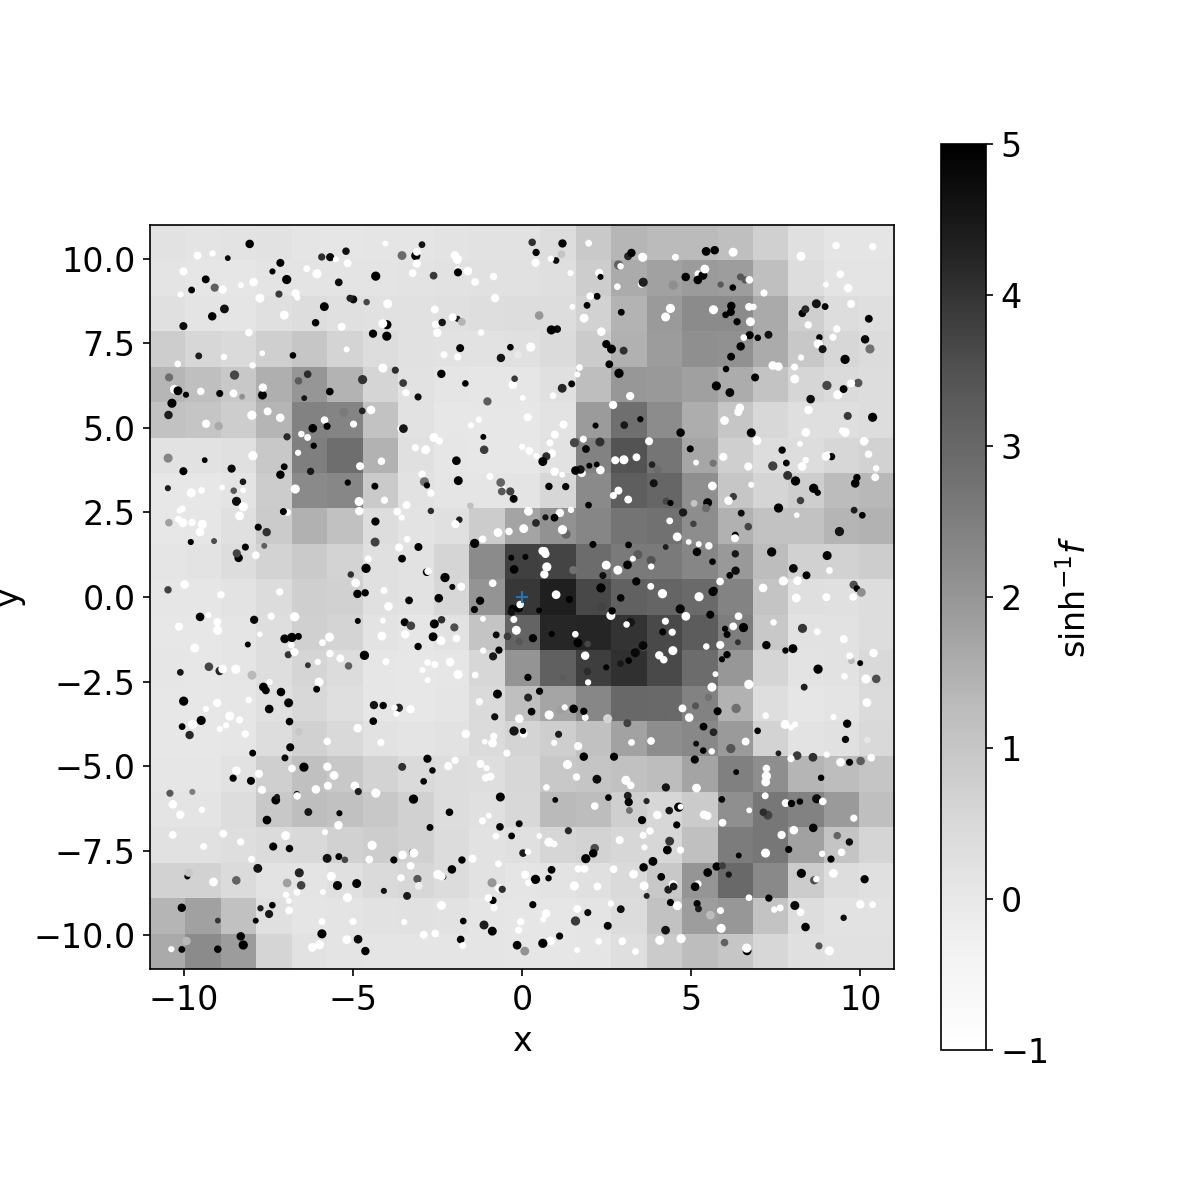
\includegraphics[width=0.24\textwidth, angle=0]
                {figures/scattered-mem-noisy.png}
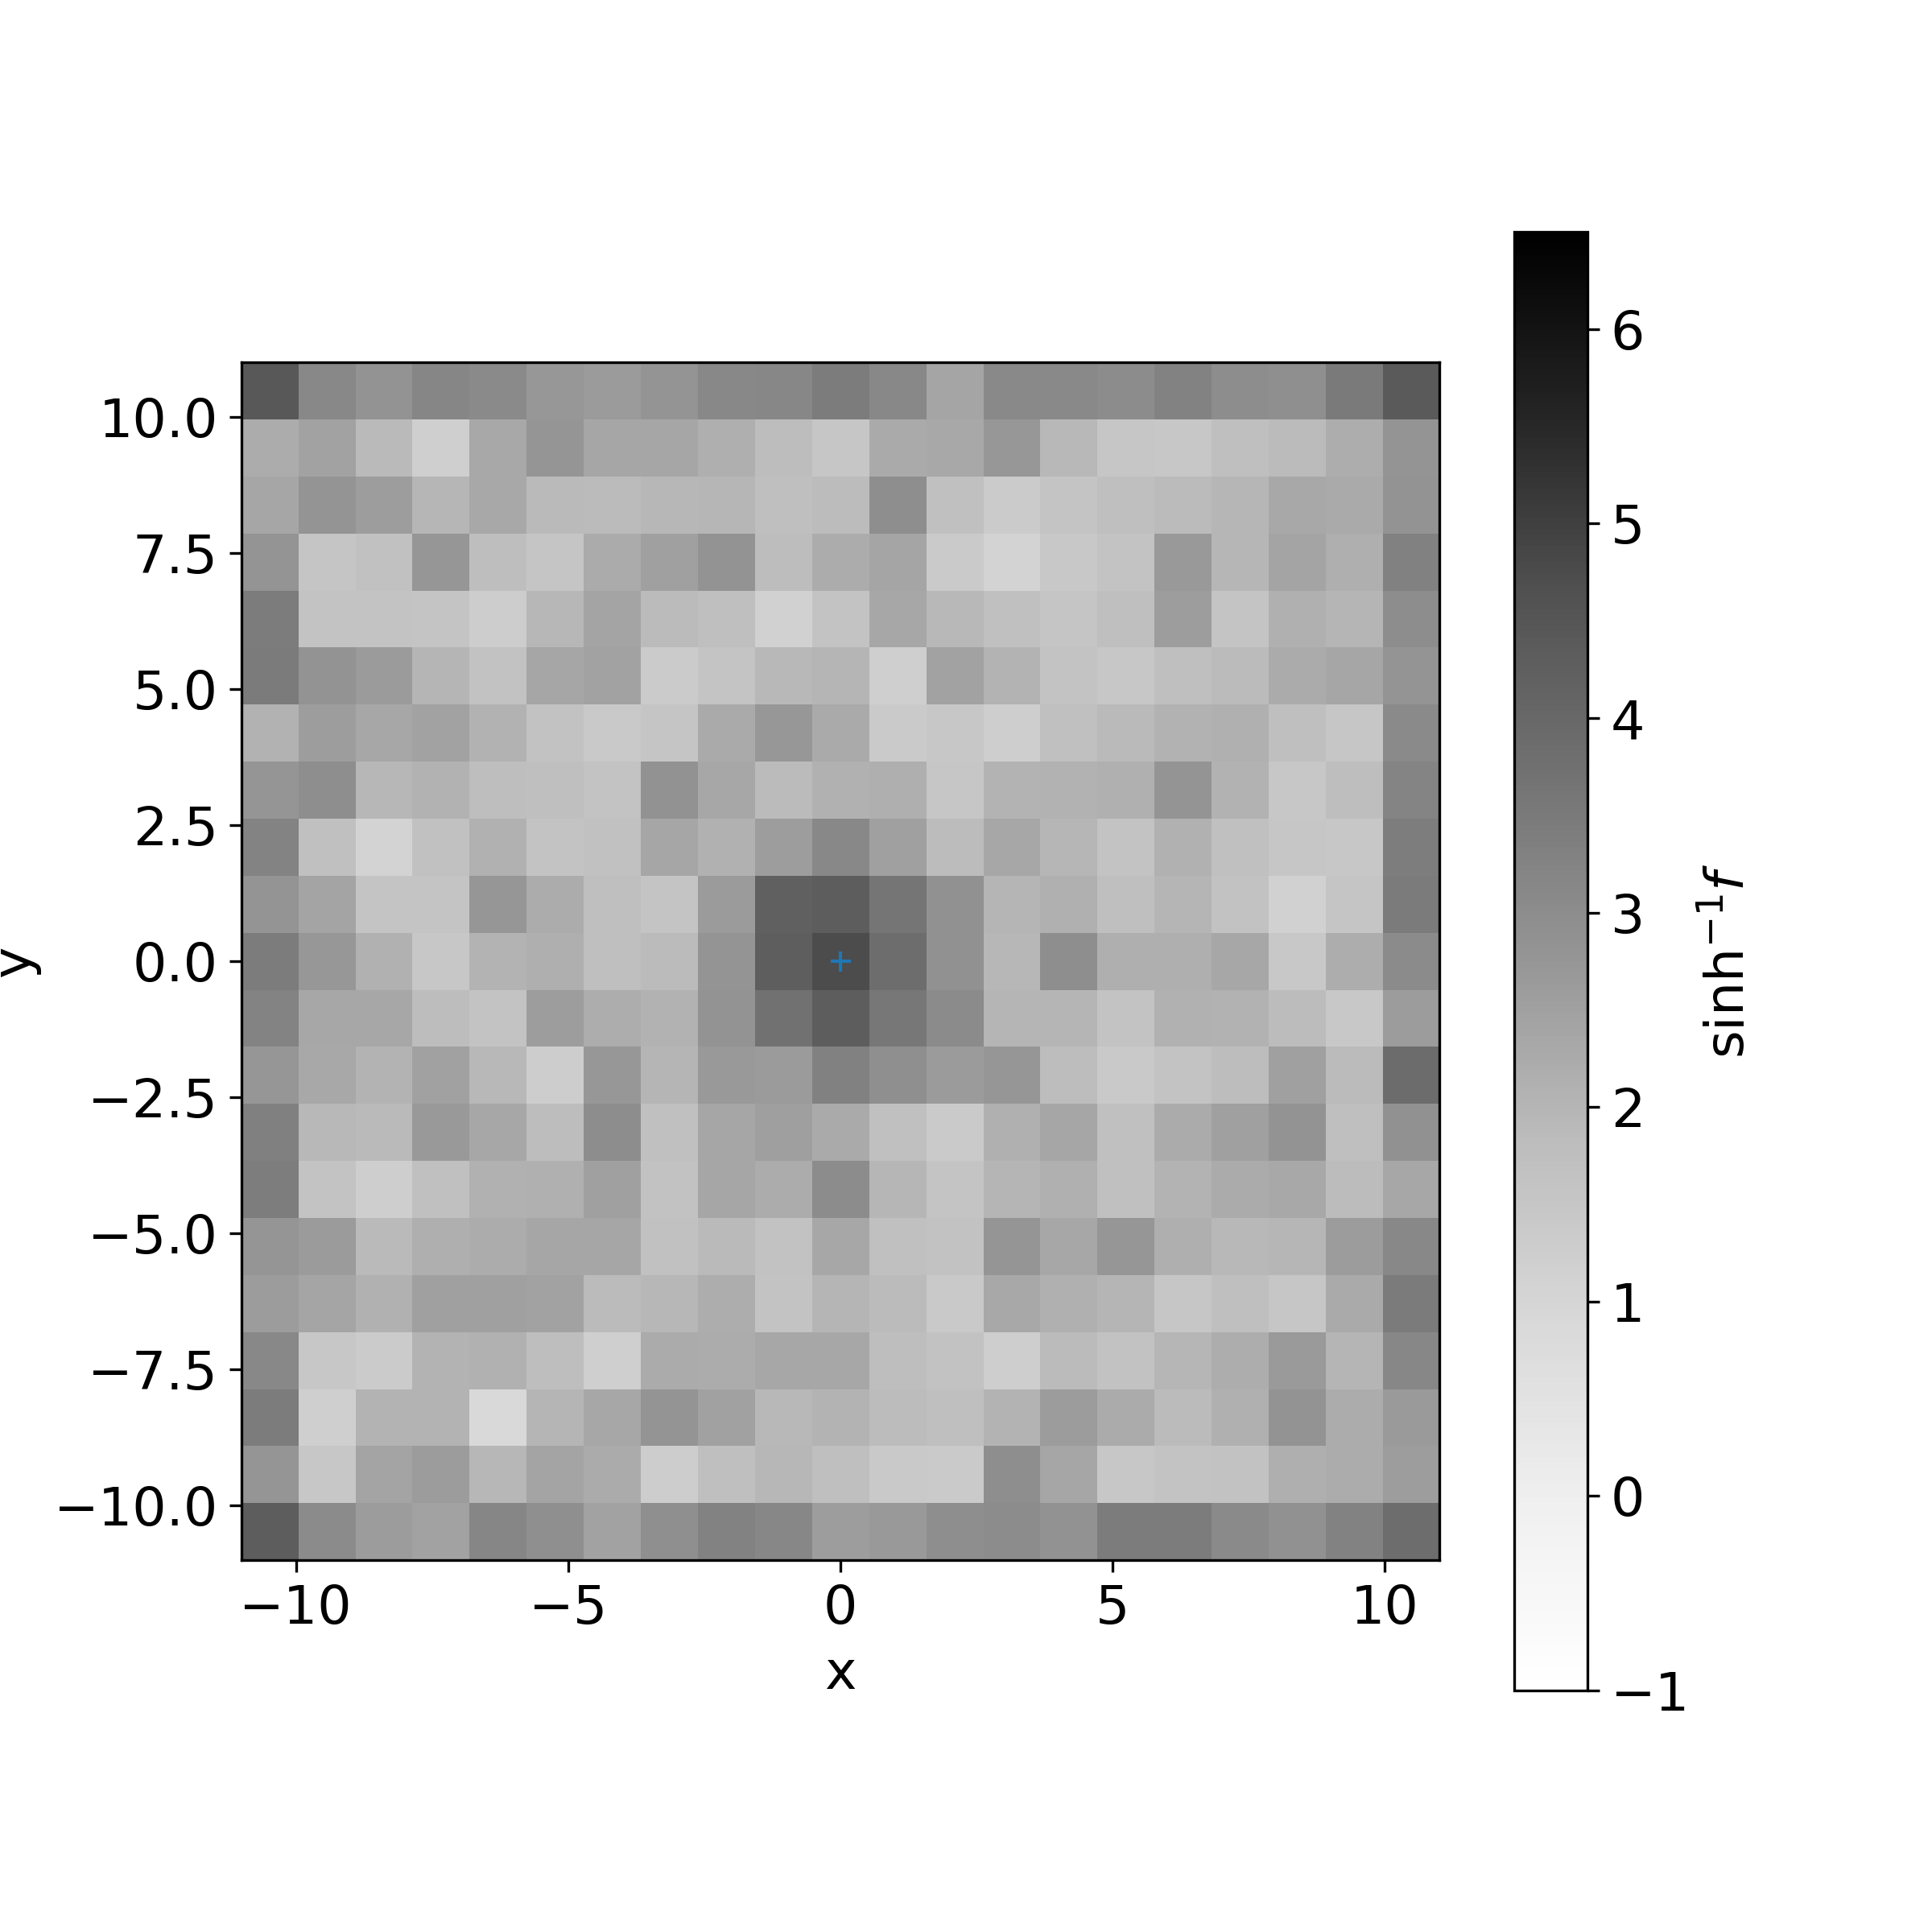
\includegraphics[width=0.24\textwidth, angle=0]
                {figures/scattered-mem-mean-100.png}
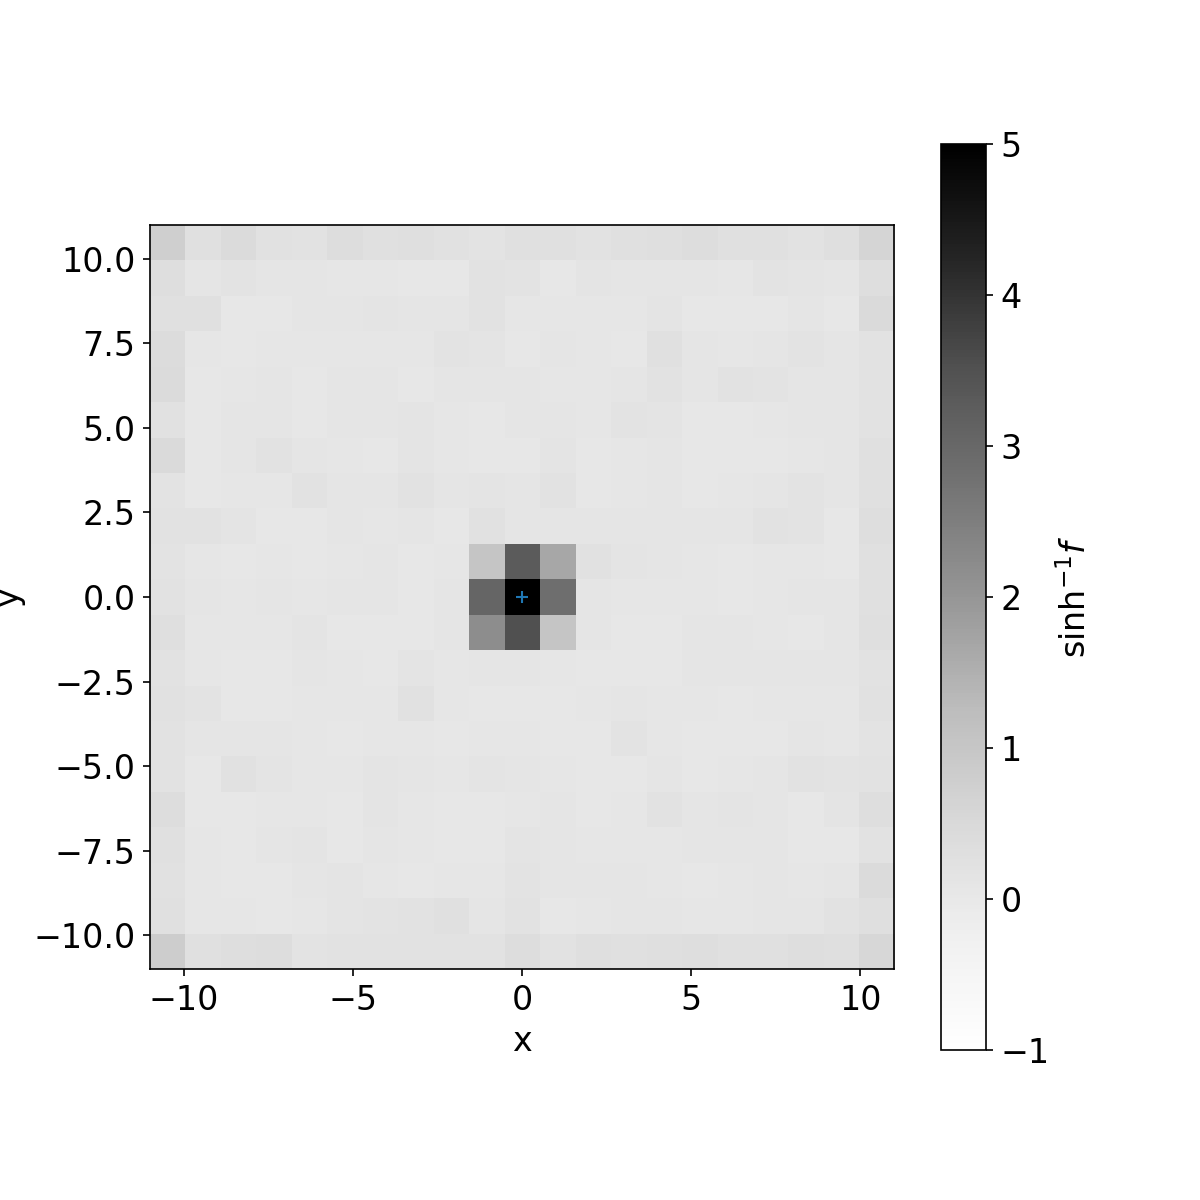
\includegraphics[width=0.24\textwidth, angle=0]
                {figures/scattered-mem-mean-1.png}
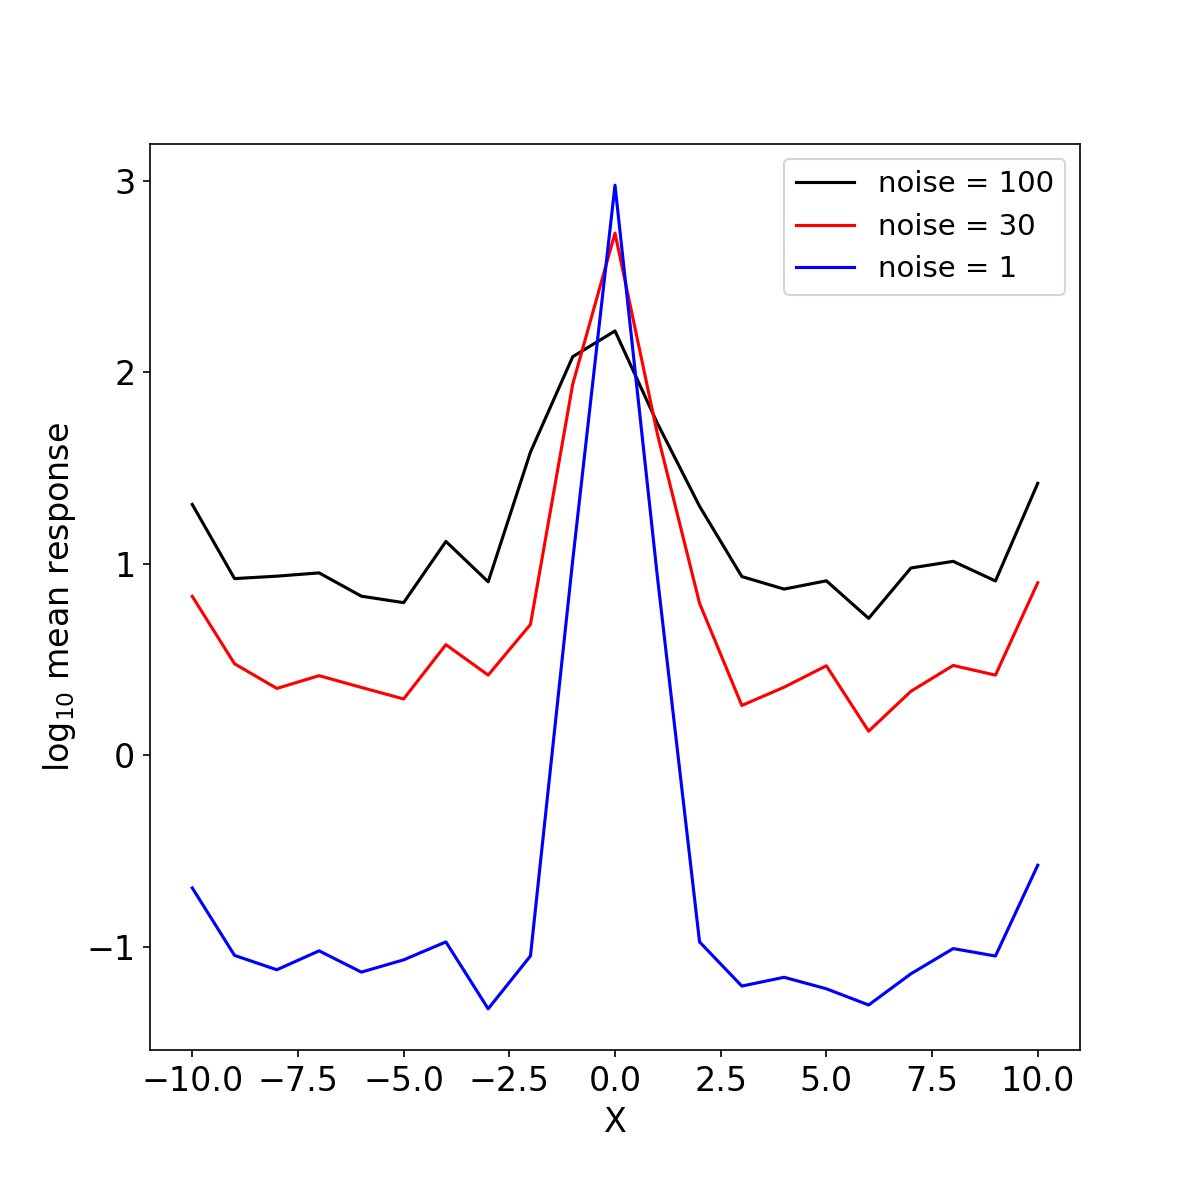
\includegraphics[width=0.24\textwidth, angle=0]
                {figures/scattered-mem-mean-slice.png}
\caption{ \label{fig:scattered-mem} Similar to Figure
  \ref{fig:scattered-nnls}, for the maximum entropy
  method applied to a point source input.}
\end{figure*} 

Figure \ref{fig:scattered-mem} shows the result of this method for
our standard point source, using $\lambda=10^{-2}$. These results do
not depend strongly on this regularization parameter. Each panel is
the same as in Figure \ref{fig:scattered-nnls}. The results are
remarkably similar, showing the same biases as the signal-to-noise
ratio decreases. These biases therefore appear to derive in large part
from the nonnegative nature of the maximum entropy method.

\begin{figure*}[t!]
\centering
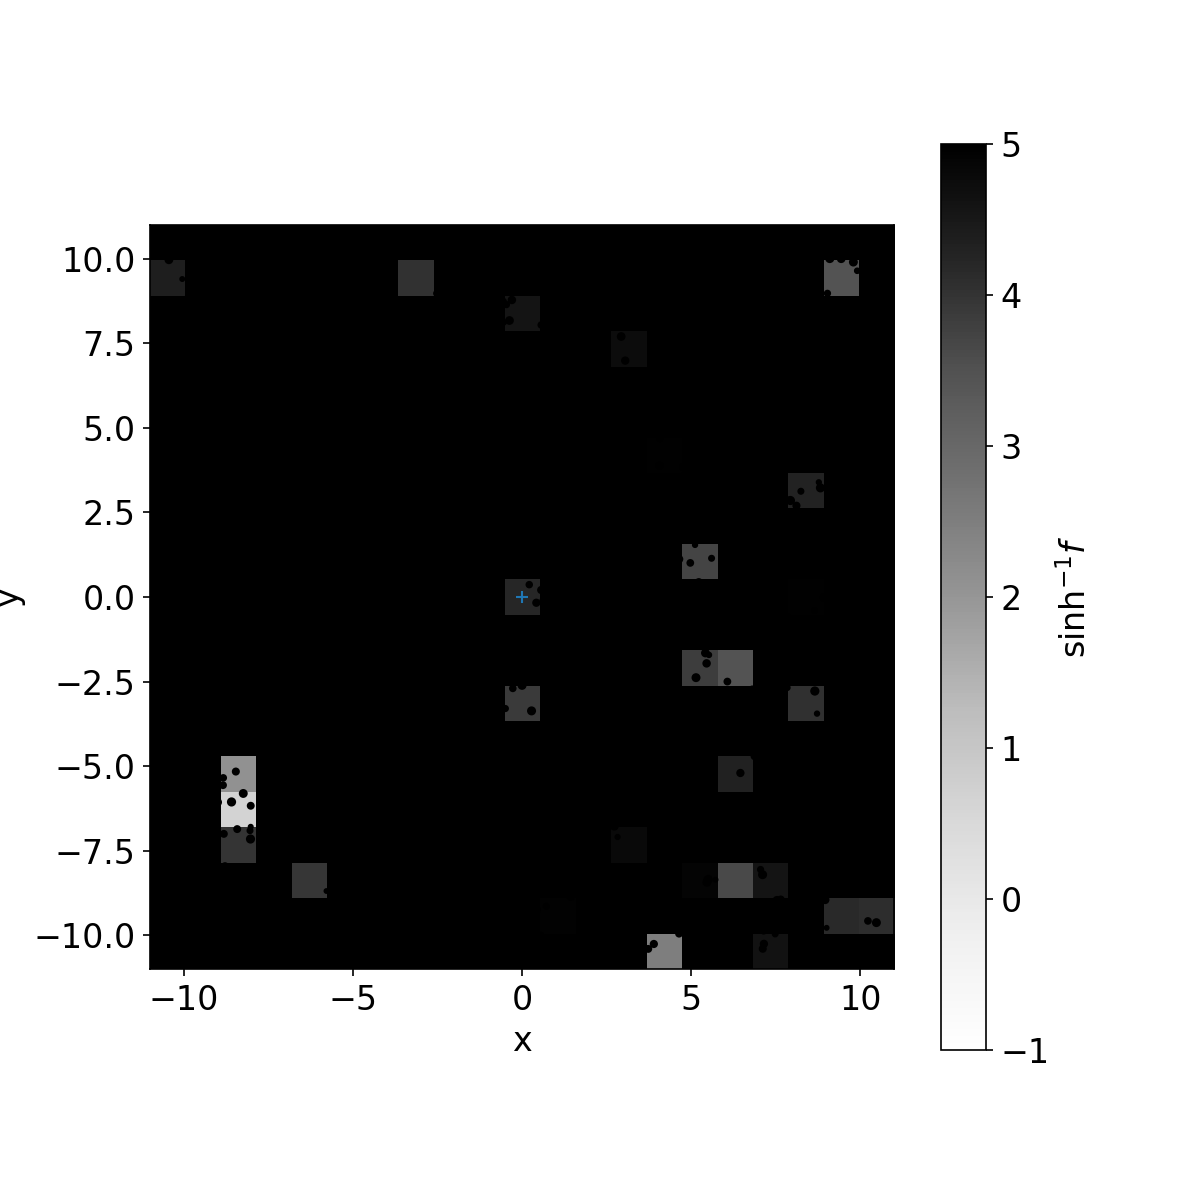
\includegraphics[width=0.24\textwidth, angle=0]
                {figures/scattered-mem-flat.png}
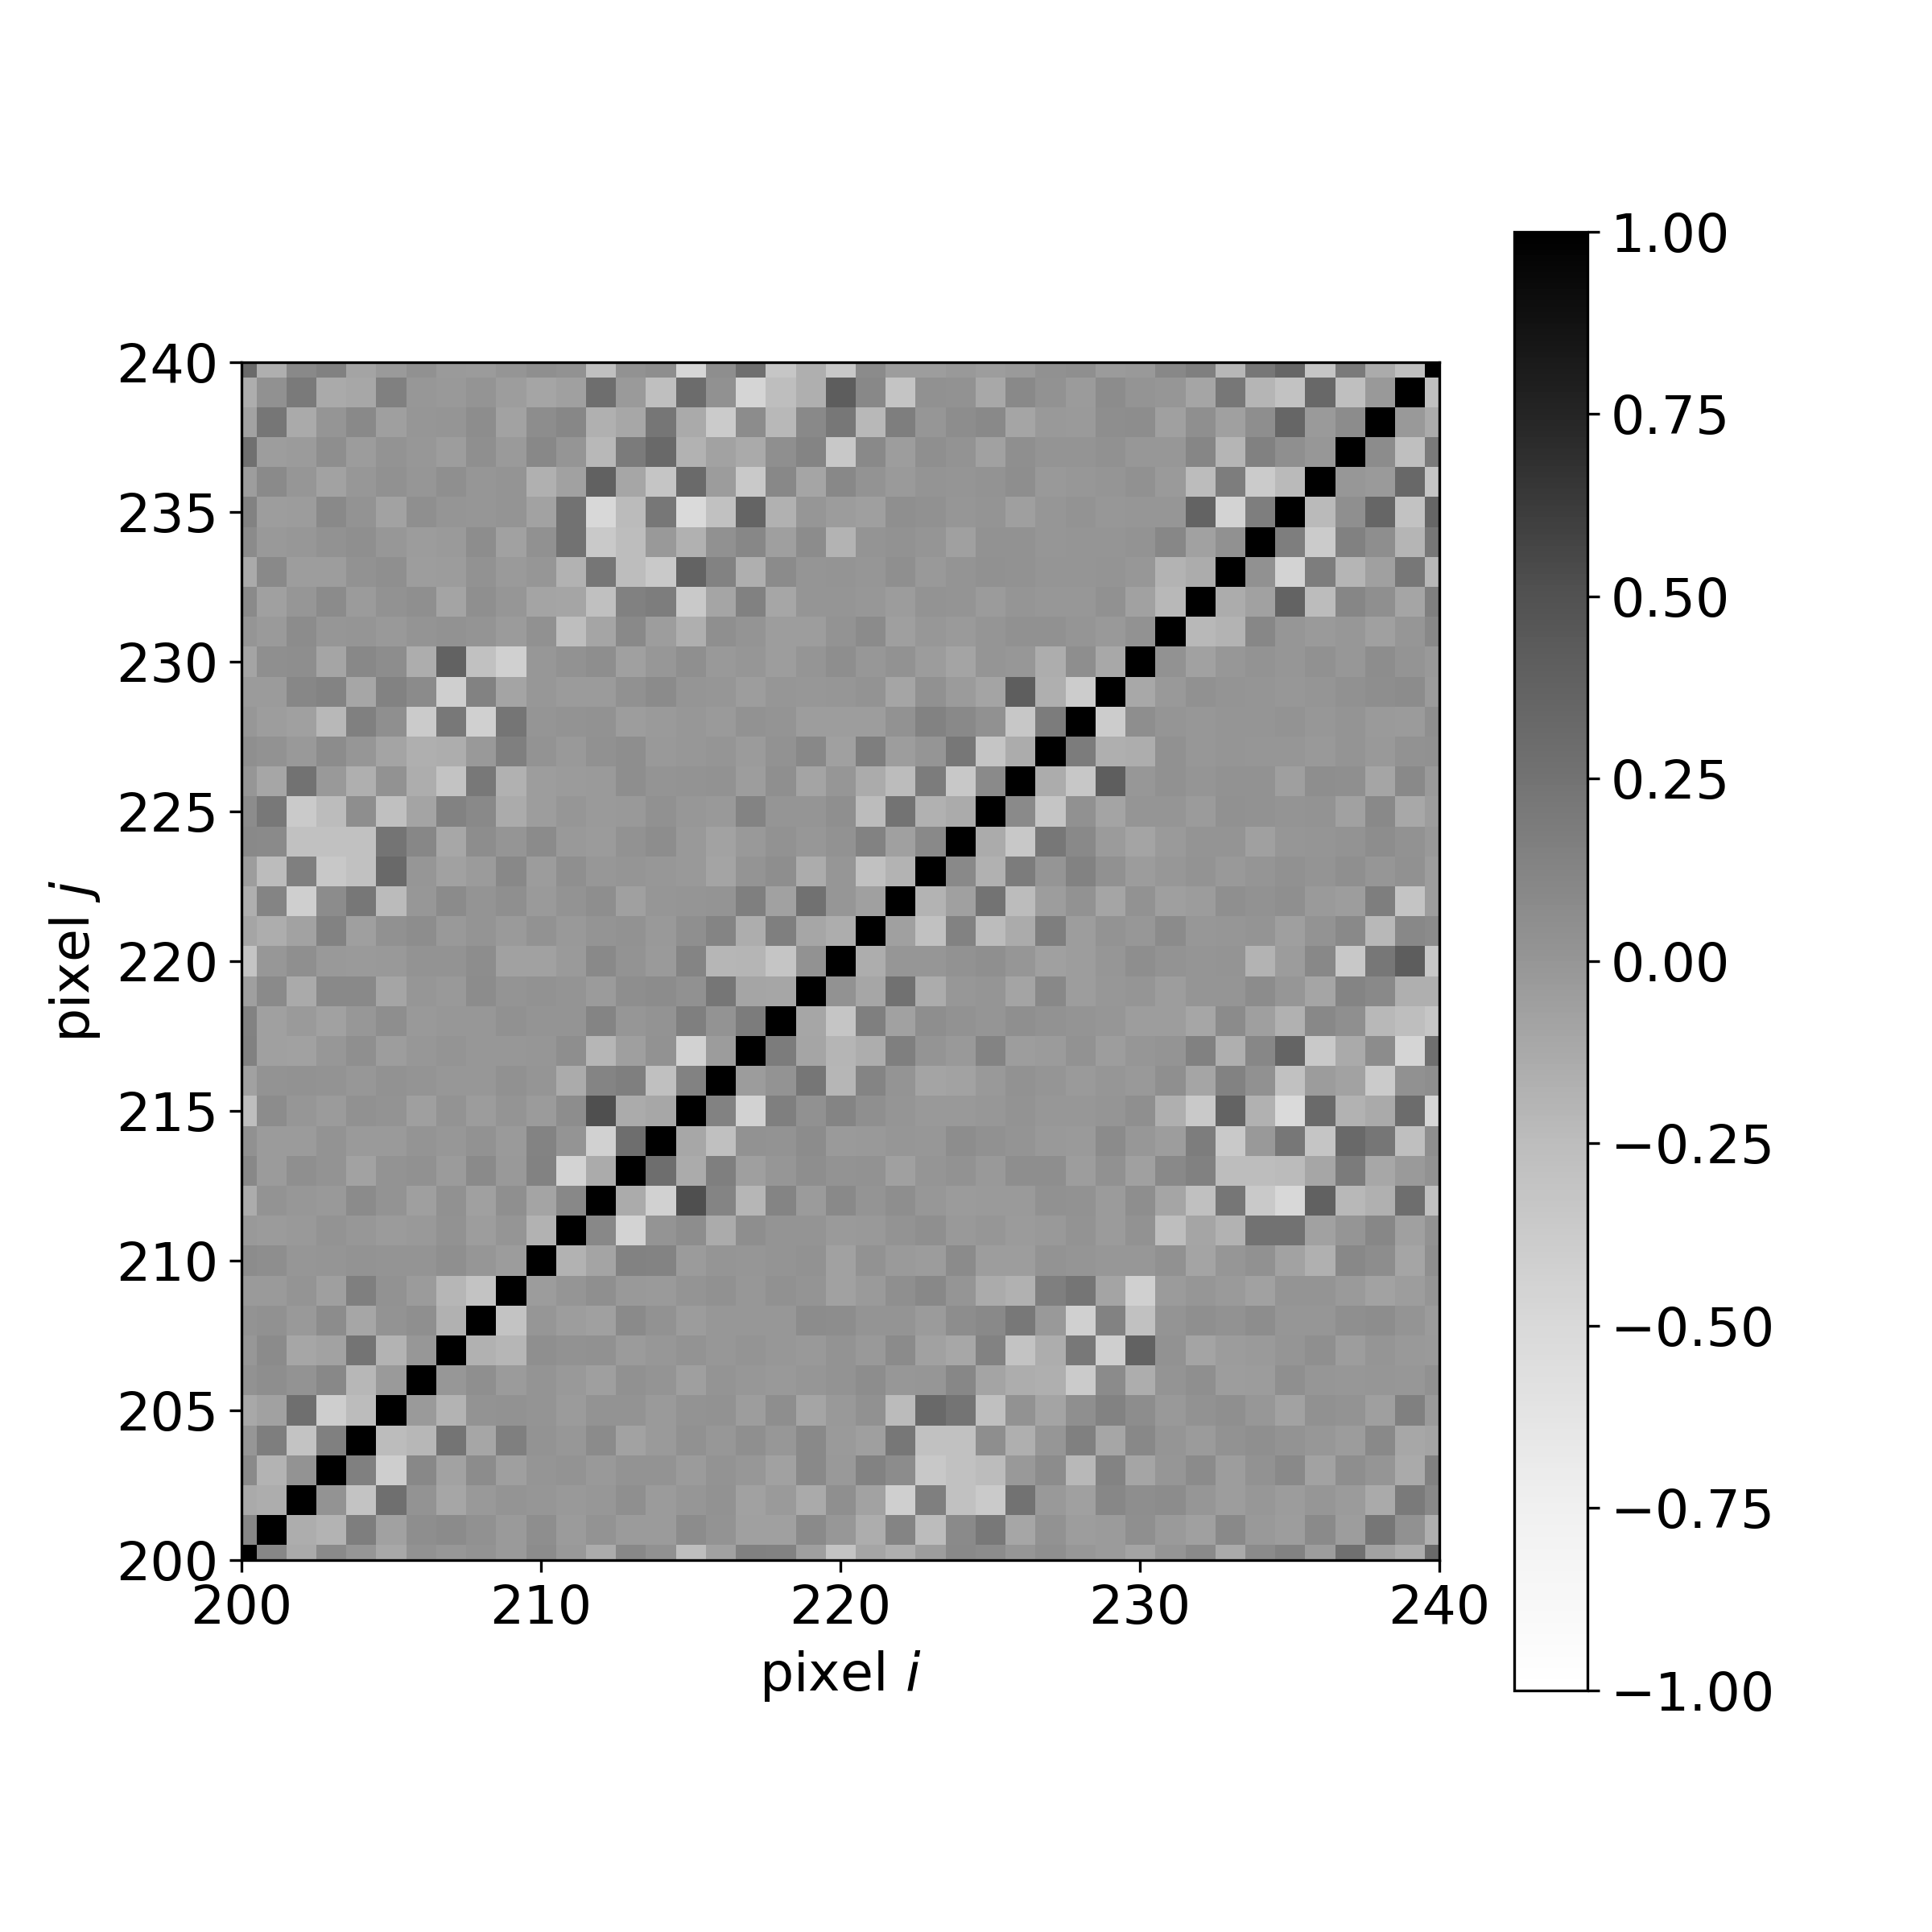
\includegraphics[width=0.24\textwidth, angle=0]
                {figures/scattered-mem-flat-covar.png}
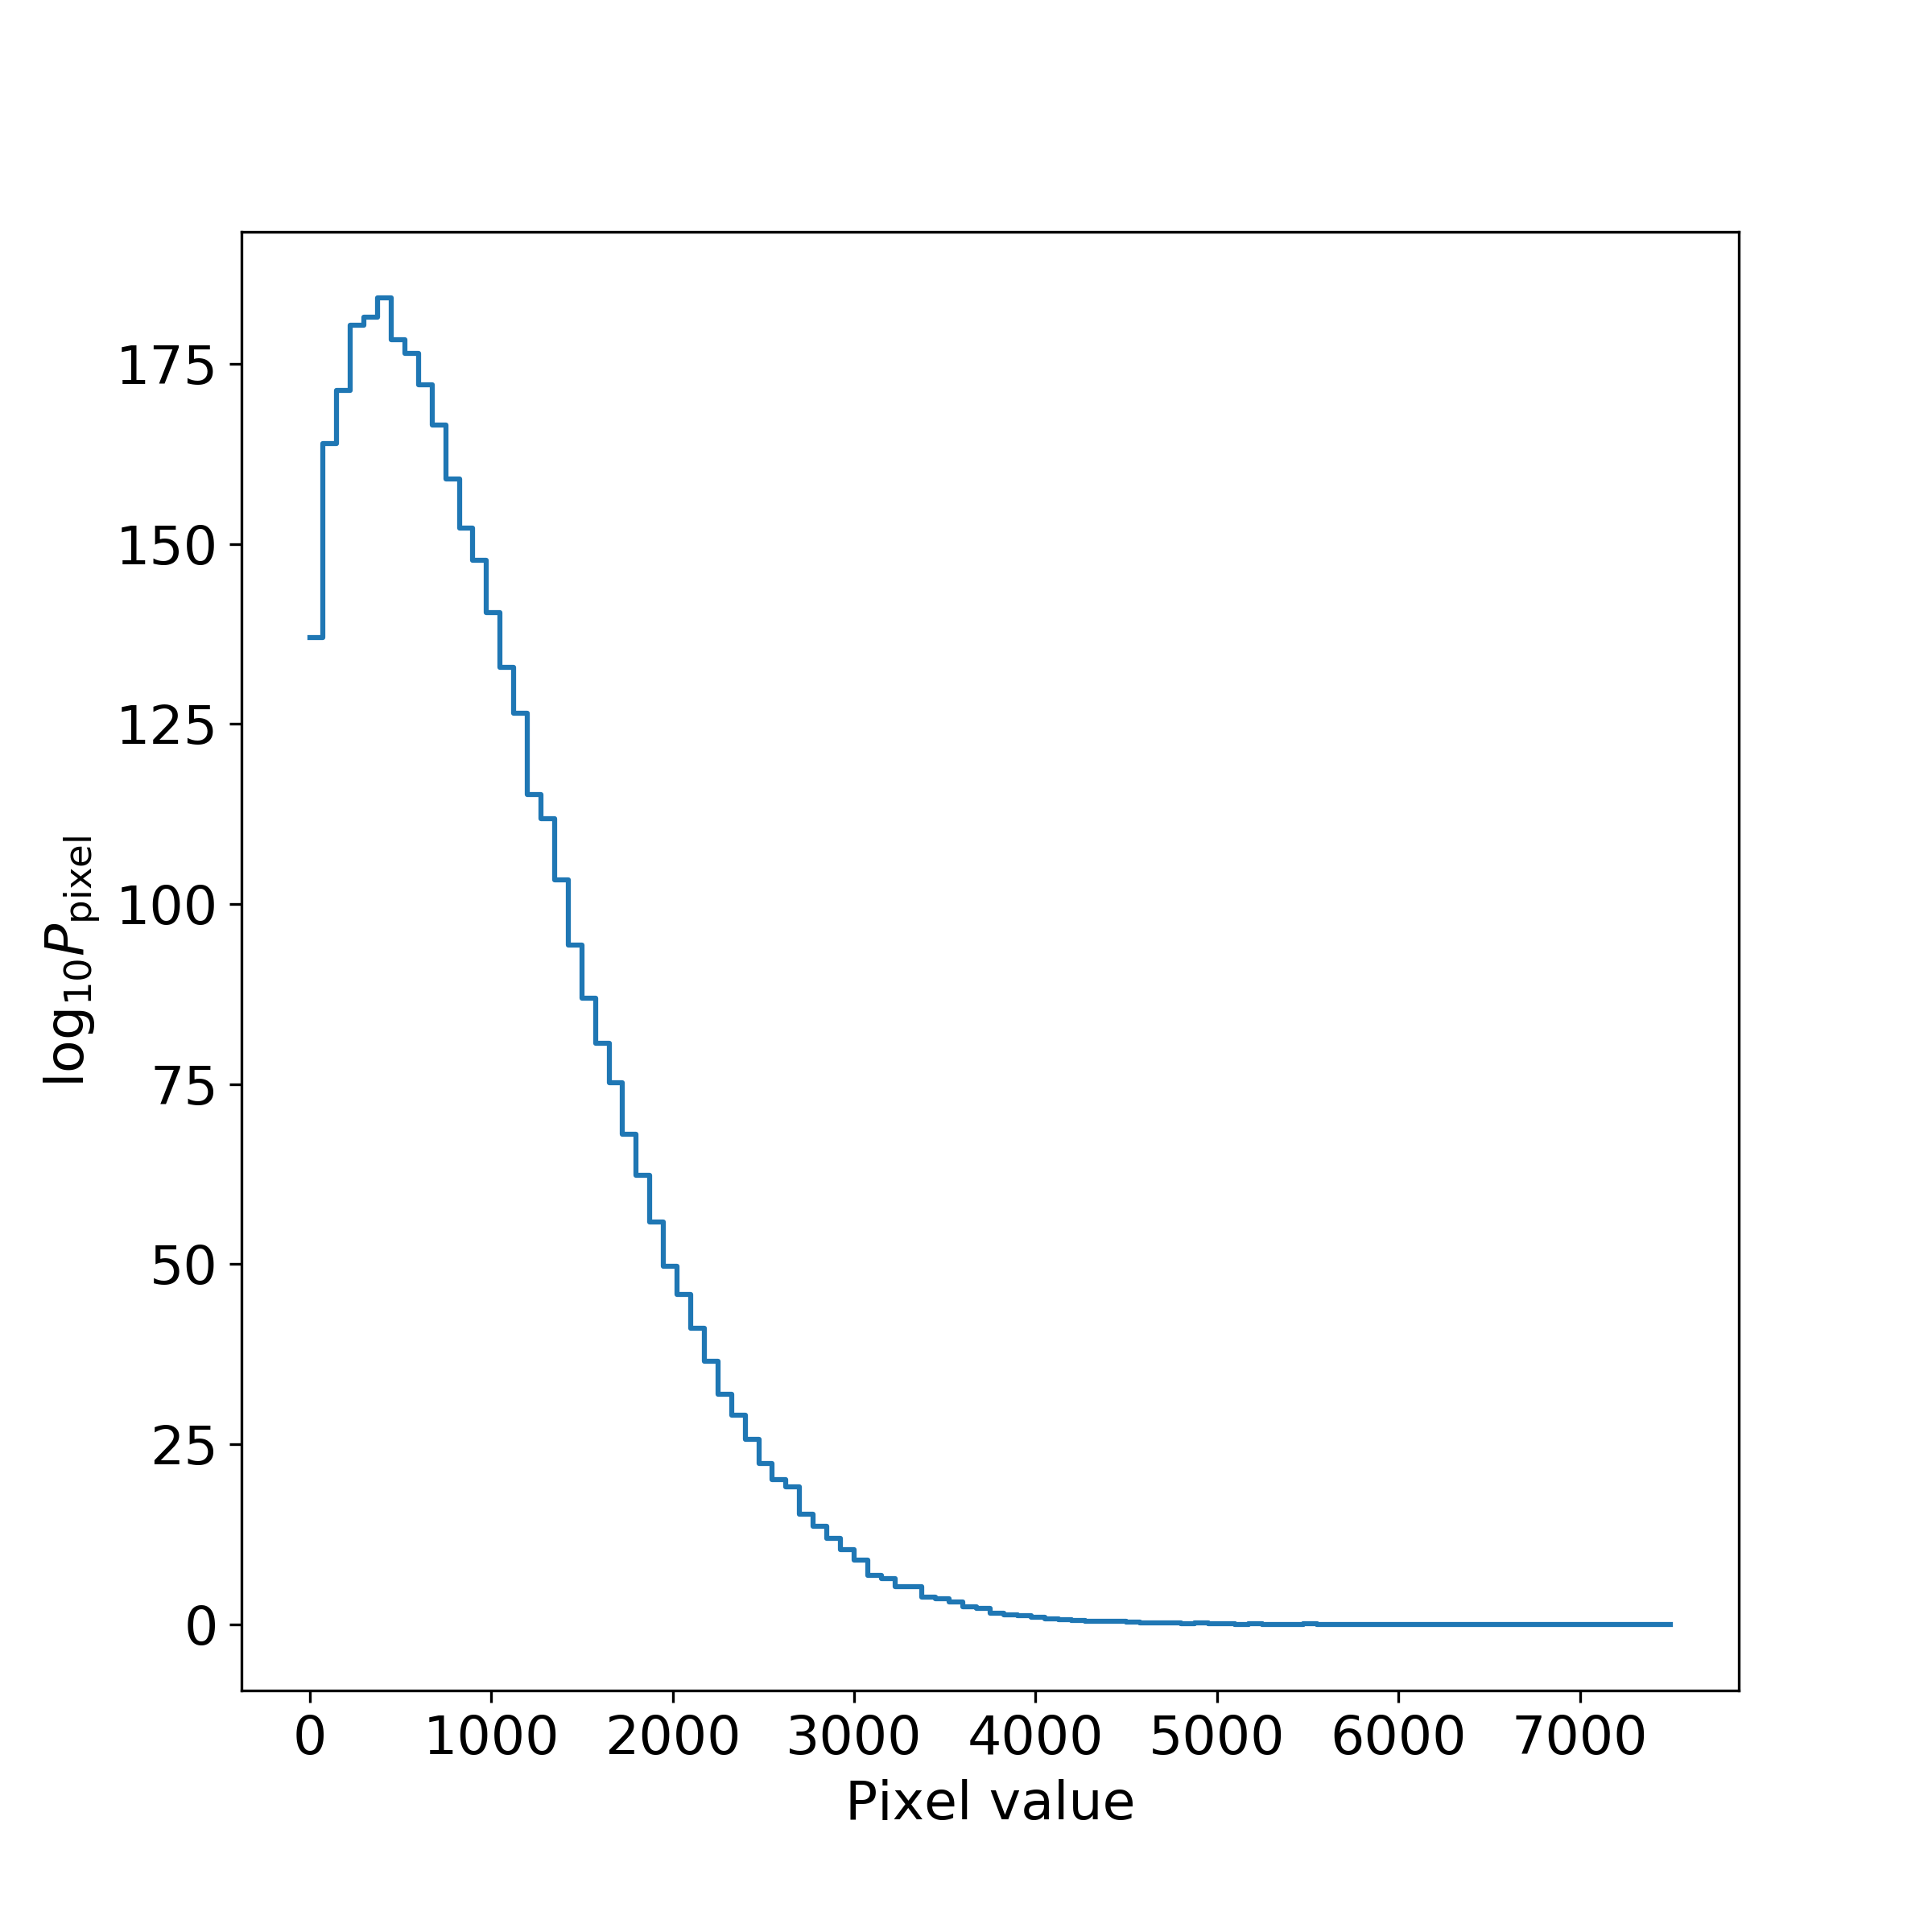
\includegraphics[width=0.24\textwidth, angle=0]
                {figures/scattered-mem-flat-dist.png}
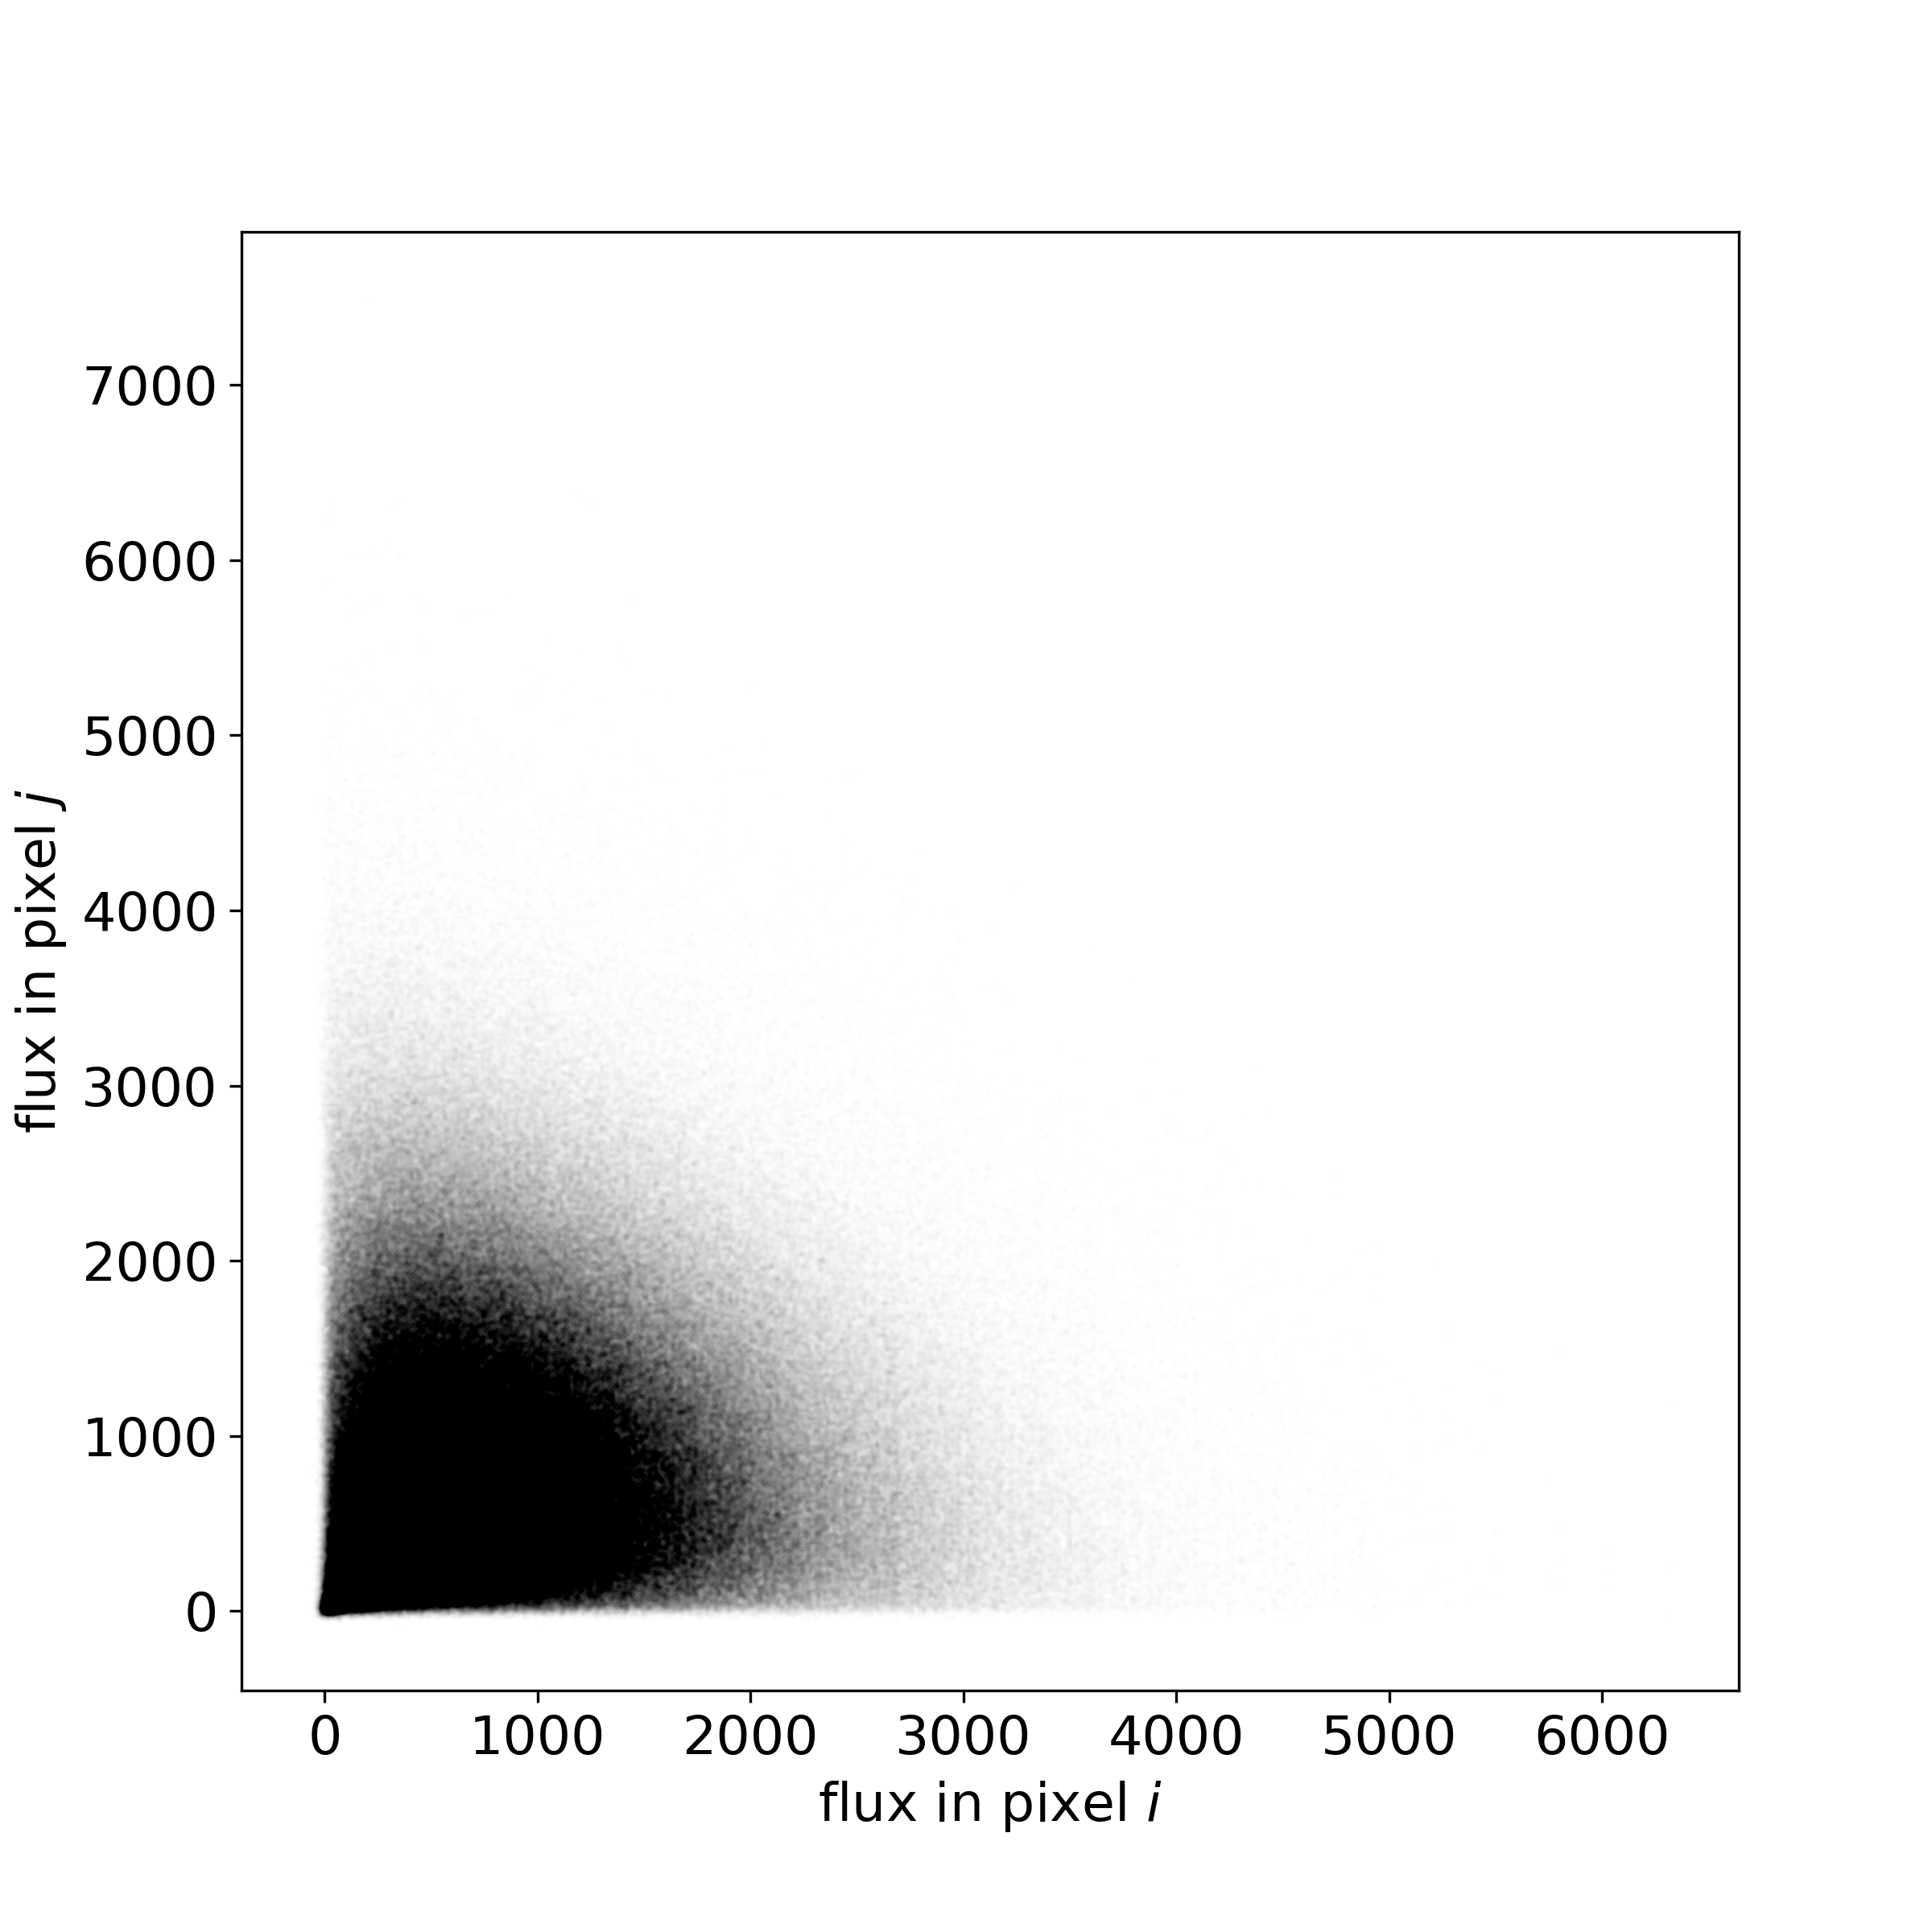
\includegraphics[width=0.24\textwidth, angle=0]
                {figures/scattered-mem-flat-dist-joint.png}
\caption{ \label{fig:scattered-mem-flat} Similar to Figure
  \ref{fig:scattered-nnls-flat} for the maximum entropy method
  applied to a uniform signal distribution.}
\end{figure*} 

Figure \ref{fig:scattered-mem-flat} shows the result of this method
for a uniform illumination, using $\lambda=10^{-2}$. In this case, the
regularization parameter matters---a much smaller $\lambda$ leads to
a result more similar to that found in Figure
\ref{fig:scattered-nnls-flat}. The resulting correlation matrix,
however, has many of the same features for maximum entropy---it is
still the case that there are anticorrelations between neighboring
pixels. In addition, the error distribution is also non-Gaussian,
though considerably less so than for nonnegative fitting.

\subsubsection{Summary}
\label{sec:deconvolution_summary}

There are many more techniques of deconvolution, tuned to and
appropriate for numerous circumstances. The very short tour above is
meant only to introduce some of the basic features of deconvolution in
the context here. The crucial features are as follows. First,
deconvolution can produce extremely sharp images. As the
signal-to-noise ratio increases, a reasonably regularized
deconvolution can produce a very sharp image. Second, the PSF of the
deconvolution tends to be either unusual (in the case of regularized
linear deconvolution) or nonexistent, with a response that is
signal-to-noise ratio dependent (in the case of nonlinear methods).
Third, many deconvolution methods require a tunable parameter whose
appropriate value depends on the data of the image being
reconstructed. Fourth, the errors in deconvolutions tend to be poorly
behaved; in all cases above, they either have strong off-diagonal
covariances or strong non-Gaussianities. The last three features mean
that there is no uniquely defined, generally applicable procedure for
deconvolution; all applications of deconvolution in the presence of
finite noise require the investigator to evaluate trade-offs in the
regularization procedure to determine what behavior is tolerable in
their application.

The point of this discussion is not to criticize any particular
application of deconvolution. Many valid and useful applications of
deconvolution exist; indeed, in many cases the problems identified in
this subsection are minor or negligible. This discussion is meant to
provide background, context, and motivation for the
covariance-regularized reconstruction described later.

\subsection{Interpolation methods}
\label{subsec:reconstructions}

Interpolation methods have perhaps less ambitious goals than
deconvolution methods. They do not seek to remove the effect of the
instrumental resolution, but seek instead to estimate the image in
between the samples. For a uniform kernel $K$, they might be
approximately described as methods that seek to infer $R(x,y)\otimes
K(x,y)$, whereas deconvolution methods seek to infer $R(x,y)$. We will
review here several reconstruction methods

\subsubsection{Shepard's method}
\label{subsec:shepard}

The method of \citet{shepard68a} or its variants are the most commonly
used for problems like our model problem; for example
\citet{sanchez12a} and \citet{law16a} use the method in the context of
integral field spectroscopy in astronomy. Many variants of this method
with different weighting function have been studied in the literature,
though they all share the essential features our simple weight
function has, namely that they are smooth, all positive, stationary
functions (\citealt{dellaccio16a}).

The basic idea is to transform the measured fluxes at each sample to
a value at each grid point using a set of linear weights:
\begin{equation}
\vec{S}_S = \mathbf{W}\cdot \vec{f}
\end{equation}
where the weights $W_{ij}$ are set using some stationary function of
the distance $r_{ij}$ between the grid point $i$ and the sample $j$.

A simple weight function is a circularly symmetric Gaussian with
standard deviation $\sigma_0$:
\begin{equation}
\label{eq:shepard_weights}
  W_{ij} = 
  \frac{1}{W_{0,i}}\exp\left(-\frac{r_{ij}^2}{2\sigma_0^2}\right),
\end{equation}
for $r_{ij} < r_{\rm lim}$, and zero otherwise. 
$W_{0, i}$ is
defined as the sum of the $N$ weights for each output grid point $i$,
to guarantee the conservation of flux:
\begin{equation}
\label{eq:shepard_norm}
W_{0, i} =\sum_{j}\exp\left(-\frac{r_{ij}^2}{2 \sigma_0^2}\right),
\end{equation}
over all pixels $i$ for which $r_{ij}< r_{\rm lim}$. 

For the model problem, Figure \ref{fig:scattered-shepard} shows the
result of Shepard's method for $\sigma_0 = 1$, given a point source
input. Since this method is purely linear, the image can be thought of
as the Point Source Function (PSF) of the experiment and method
combination.

\begin{figure}[t!]
\centering
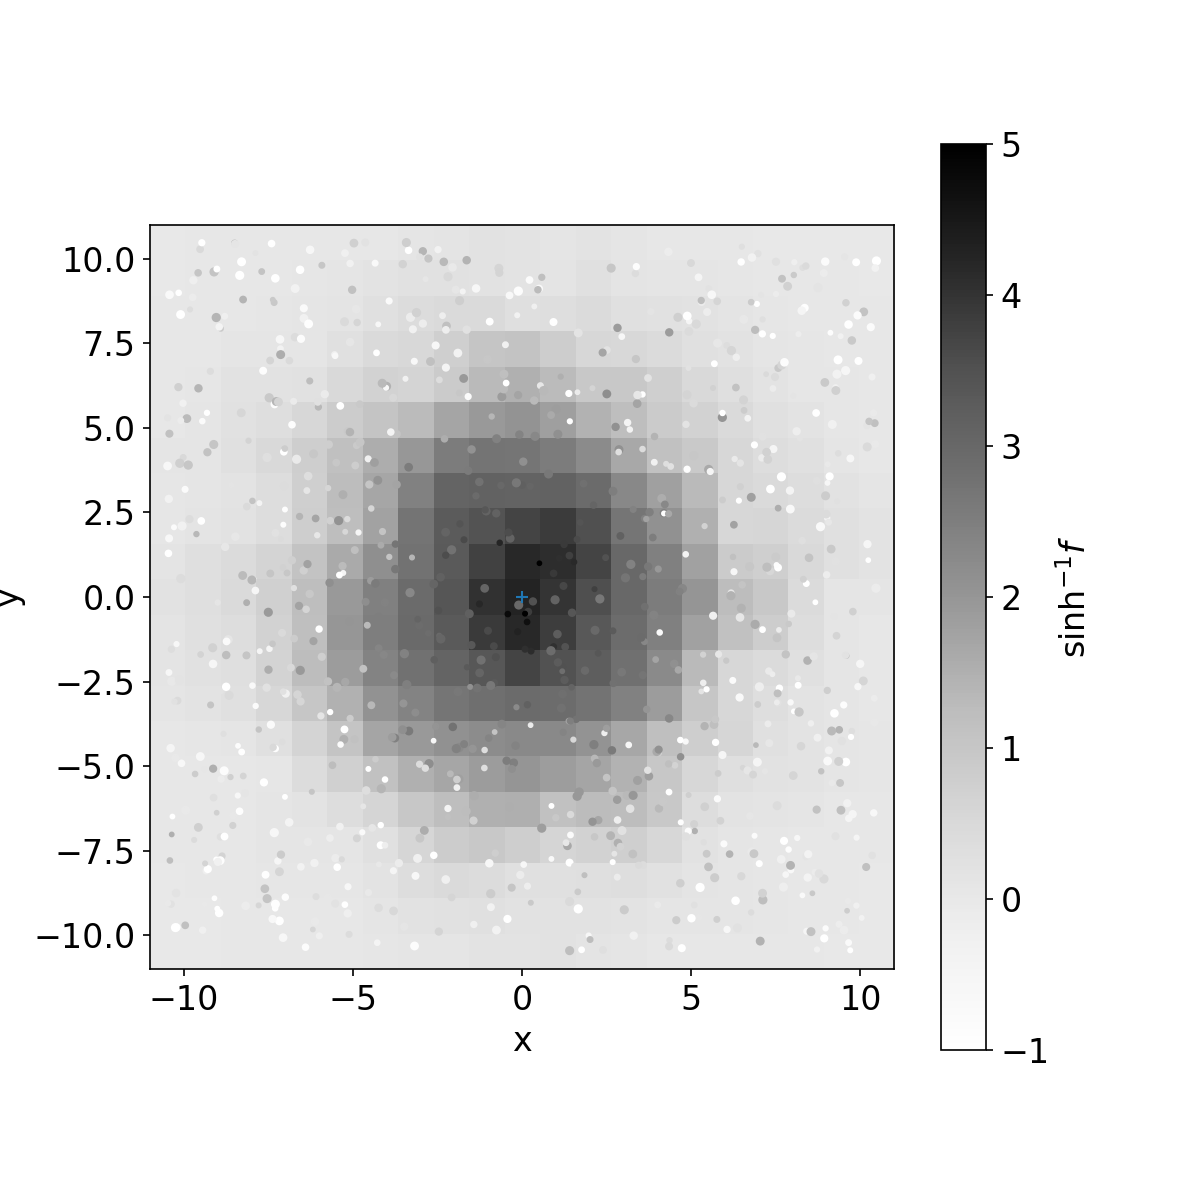
\includegraphics[width=0.23\textwidth, angle=0]
                {figures/scattered-shepard.png}
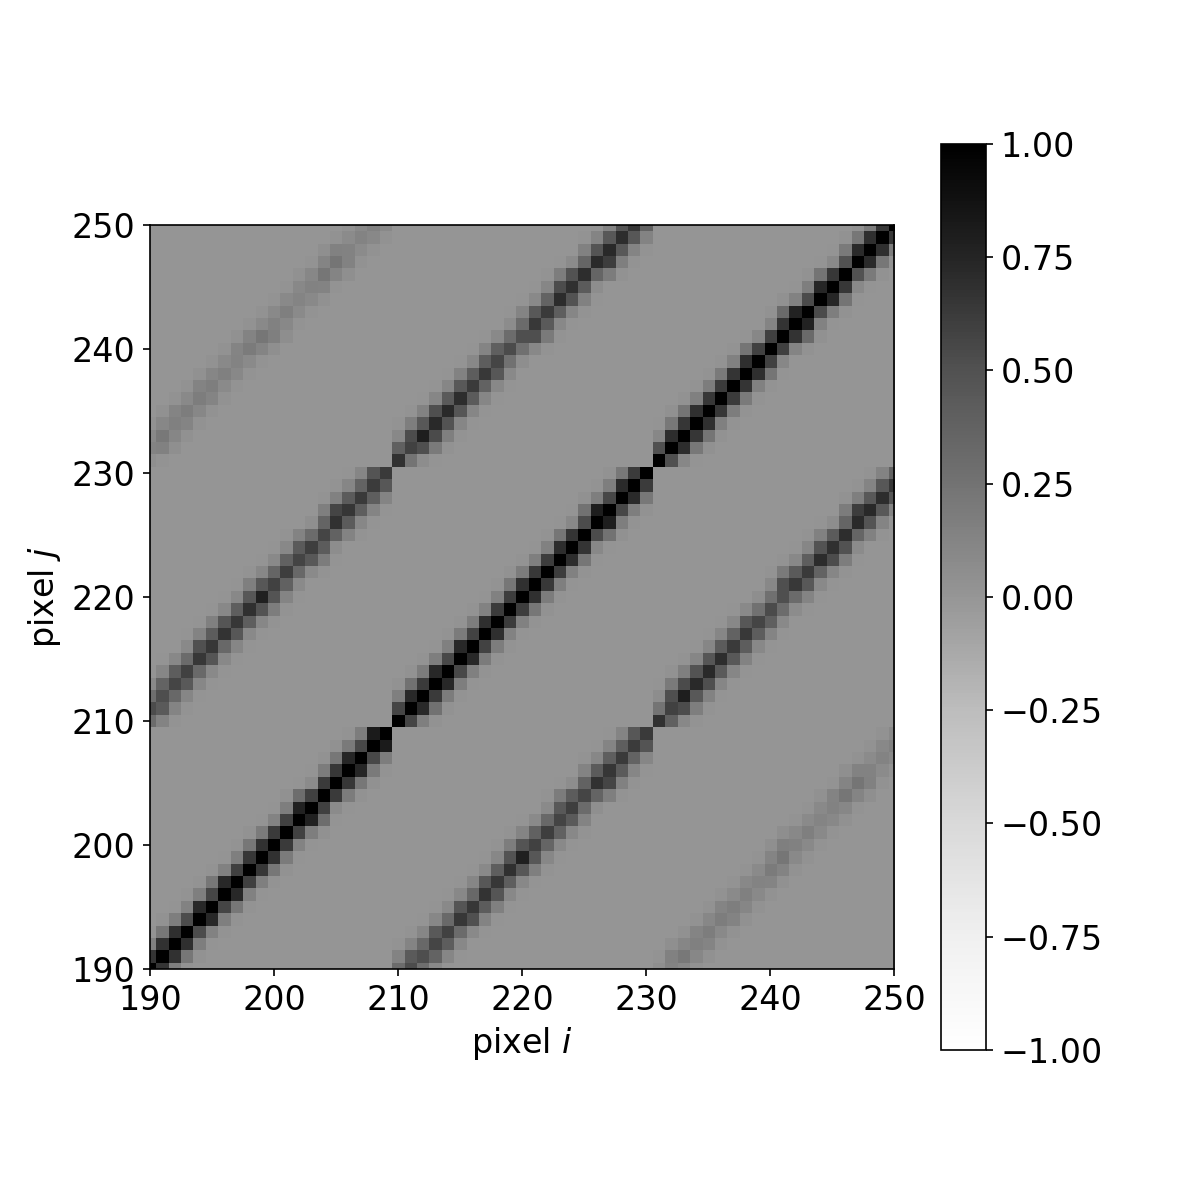
\includegraphics[width=0.23\textwidth, angle=0]
                {figures/scattered-shepard-covar.png}
\caption{ \label{fig:scattered-shepard} {\it Left panel}: Shepard's
  method for noiseless case. {\it Right panel}: Subsection of the
  covariance matrix of Shepard's method.}
\end{figure} 

Obviously the PSF for Shepard's method is much broader than for the
deconvolution methods, by construction. It reflects both the
resolution of the kernel and to some extent the choice of the weights
$W_{ij}$. In our test case, the resolution of the kernel is variable,
so its exact effect is unclear. Therefore, we tested the effect of
Shepard's method on the resolution by testing a case with a constant
kernel. We found that the best-fit Gaussian width $\sigma_{\rm PSF}$
of the PSF was well-approximated by the combination in quadrature of
the kernel width $\sigma$ and the $\sigma_0$ used by Shepard's
method. We conclude that Shepard's method tends to degrade the image 
relative to the kernel-convolved image.

In addition, Shepard's method exhibits a broad non-diagonal
correlation matrix. In this case, unlike the deconvolution, there are
positive correlations between neighboring pixels instead of negative
ones. This correlation is caused by the fact that errors in the
samples will affect neighboring pixels in very similar ways; if a
sample fluctuates upward or downward, a bunch of neighboring pixels
fluctuate upward or downward together.

\subsection{Gaussian Process Regression}
\label{sec:gp}

\section{Covariance-Regularized Reconstruction}

In this paper, we present a different approach to reconstruction,
whose goals and methods are informed by the previous methods discussed
above. Like the model-fitting approaches discussed above, we seek a
reconstructed image that is consistent with all of the input
data. However, instead of regularizing the values of the
fully-deconvolved images, the method reports a reconstructed image
equal to the fully-deconvolved image, reconvolved with a point spread
function designed so that each reported pixel value is statistically
independent. That is, we desire that the covariance matrix of the
pixel values is diagonal.

This goal has the following implications:
\begin{itemize}
\item The pixel values do not have the anticorrelations that are
  present in the full deconvolution. This  fact leads to a smooth
  image that avoids the amplification of noise.
\item The resulting image can be analyzed without accounting for
  off-diagonal covariances, which simplifies subsequent analysis. 
\end{itemize}

Like some of the techniques above, it involves constructing a
model that explains all of the data. However, instead of regularizing
that model through smoothness, nonnegativity, or entropy criteria, we
regularize the covariance between pixels in our outputs
model. Specifically, we seek a method that guarantees zero
off-diagonal covariance. The resulting image is related to the true
deconvolved image through a known PSF; indeed, the result is very
similar to performing a full deconvolution and then reconvolving with
the native resolution.

We begin with the covariance of the fully deconvolved image
$\vec{S}_F$:
\begin{equation}
  \mathbf{C}_F = \mathbf{V}\cdot \mathbf{\Sigma}^{-2} \cdot \mathbf{V}^T
\end{equation}
We seek to linearly transform $\vec{S}_F$ into a new quantity
$\vec{S}_G$ with the property that its covariance matrix is diagonal
if the input values $\vec{f}$ also have a diagonal covariance matrix.

It is straightforward to verify that the matrix $\mathbf{V}$ consists
of the eigenvectors and $\mathbf{\Sigma}^{-2}$ of the eigenvalues of
the covariance $\mathbf{C}_F$. The transformation $\mathbf{V}^T \cdot
\vec{S}_F$ therefore will yield a vector whose covariance is
diagonal. However, this new vector would redistribute the signal into
a set of modes sorted by variance. Whereas each entry in $\vec{S}_F$
is associated with a pixel in the image, each entry in
$\mathbf{V}^T\cdot\vec{S}_F$ would be some combination of pixels
without any necessary geometric relationship with the pixel associated
with the corresponding entry in $\vec{S}_F$.

Instead consider the following transformation:
\begin{equation}
\label{eq:resolution}
  \mathbf{R} = \mathbf{Q}_S \cdot \mathbf{Q} =
  \mathbf{Q_S} \cdot \mathbf{V}\cdot \mathbf{\Sigma} \cdot\mathbf{V}^T,
\end{equation}
where $\mathbf{Q}_S$ is any diagonal matrix and $\mathbf{Q}$ can also
be interpreted as the inverse of the square root of the covariance
matrix:
\begin{equation}
\mathbf{C}_F = \mathbf{Q}^{-1} \cdot \mathbf{Q}^{-1}.
\end{equation}
From right to left, the operator $\mathbf{R}$ in Equation
\ref{eq:resolution} first uses $\mathbf{V}^T$ to rotate $\vec{S}_F$
into a space where the covariance is diagonal. Then it rescales each
axis in this space by $\mathbf{\Sigma}$, which makes the covariance
matrix the identity matrix. Then it uses $\mathbf{V}$ to rotate back
to the original axes. This orients the vector such that its entries
may be associated directly with the original pixels. Because the
covariance has been ``whitened,'' i.e. made spherically symmetric by
multiplying by $\mathbf{\Sigma}$, prior to the rotation back, the
covariance remains diagonal. Thus, the net transformation is to
rescale the vector along the principal axes of the covariance matrix.

Because $\vec{S}_F$ is meant to represent an image, this rescaling can
change properties of the result that we would like instead to remain
unchanged; for example, we expect that our transformation should not
add or subtract signal from the image, but the tranformation
$\mathbf{V}\cdot \mathbf{\Sigma} \cdot\mathbf{V}^T$ will in general do
so. Luckily, we may multiply by any diagonal matrix $\mathbf{Q}_S$ and
the covariance remains diagonal. We thus define
\begin{equation}
Q_{S, ij} = \frac{\delta_{ij}}{\sum_{j'} Q_{ij'}}.
\end{equation}
Then $\mathbf{Q}_S$ has the property that the flux in $\vec{S}_F$ is
conserved.

We then see that:
\begin{eqnarray}
  \vec{S}_G &=& \mathbf{W}_G \cdot \vec{f} \cr
  &=& \mathbf{R} \cdot \mathbf{W}_F \cdot \vec{f} \cr
  &=& 
  \mathbf{Q_S} \cdot \mathbf{V}\cdot \mathbf{\Sigma}
  \cdot\mathbf{V}^T \cdot \mathbf{V} \cdot \mathbf{\Sigma}^{-1}\cdot
  \mathbf{U}^T \cdot \mathbf{N}^{-1/2} \cdot \vec{f}\cr
  &=& 
  \mathbf{Q_S} \cdot \mathbf{V}\cdot 
  \mathbf{U}^T \cdot \mathbf{N}^{-1/2} \cdot \vec{f}
\end{eqnarray}
and then we can show:
\begin{equation}
C_{G, ij} = Q_{S, ij}^2 \delta_{ij}.
\end{equation}
As we will show explicitly below, $\mathbf{R}$ represents the PSF of
the resulting image; if the native PSF is constant among the samples,
it is equal to that. 

One issues arises with this method as described, which is that because
$\mathbf{N}^{-1}$ enters the procedure, the PSF depends on the noise
estimate. If the noise estimate depends on the signal itself (for
example because the image is the result of a Poisson process) then the
recovered PSF is a function of the signal, which in many applications
is undesirable. Therefore, we recommend replacing $\mathbf{N}^{-1}$ with
$\mathbf{\tilde N}^{-1}$, defined to be 1 if $\mathbf{N}^{-1}$ is
greater than zero and 0 if $\mathbf{N}^{-1}$ is equal to zero.

This method has an interesting relationship with interpolation methods
for regular grids. Nyquist-sampled images on rectangular grids (or
images that are easily deformable to rectangular grids) can be
perfectly interpolated using a sinc kernel. Under a pure shift
(i.e. not under a rotation, scale, or other deformation), and for
constant noise with a diagonal covariance, the shifted image also has
a diagonal covariance matrix. Strictly, these properties hold only for
images infinite in size.  Note that usually sinc interpolation is
modified in practice by damping the kernel at large radius. As we show
in the Appendix, the covariance-regularized reconstruction method
described above is identical to sinc interpolation for pure shifts in
the limit of infinite size images of constant noise.

This method is also closely related to the construction of ``proper''
image coadds from individual images of varying PSF, as described by
\citet{zackay17a}. {\bf NEED TO DO THE MATH AND SEE IF THIS IS TRUE}.

Although we relegate the lengthy proofs of these statements to the
Appendix, in both cases the perhaps surprising result is ultimately a
consequence of the properties of the SVD of circulant
matrices. Specifically, the eigenvectors of such matrices are the
discrete Fourier modes. This property yields an analytic result for
the SVD and for the weights $\mathbf{W}_G$ under a shift.  {\bf BUT
  UNCLEAR WHERE IT COMES FROM FOR PROPER COADDS}.

\section{Summary}
\label{sec:summary}

\acknowledgments

We thank people. David W. Hogg. Robert H. Lupton. Mike O'Neil. Adam
S. Bolton. David J. Schlegel. David R. Law.

\appendix

\section{Sinc interpolation and covariance-regularized reconstruction}

Sinc interpolation is interpolation from a uniform grid using the kernel:
\begin{equation}
\sinc\left(\frac{x}{\Delta}\right) = \frac{\sin \left(x /
  \Delta\right)}{x / \Delta} 
\end{equation}
where $\Delta$ is the grid spacing. The two-dimensional version of
sinc interpolation is simply the one-dimensional version applied
separately in each dimension.

For infinitely large, perfectly Nyquist-sampled images, sinc
interpolation is perfect---the original image samples fully specify
the sampled function, and the sinc interpolation method perfectly
reproduces it. Under the same conditions, plus the condition of
constant noise with a diagonal covariance (that is, no noise
correlation between pixels), then if you shift an image using sinc
interpolation, the noise in the resulting image has the same noise as
the original pixels and still has a diagonal covariance. This last
property does not hold for rotations, rescalings, or other
deformations of the image.

In practice, sinc interpolation is usually modified by damping the
kernel at large scales. Doing so can limit the effects of artifacts
due to the image not being Nyquist sample or having varying noise
(most particularly, if extreme value parts of the image have larger
noise, which can cause ``ringing'' in the result). However, in this
Appendix we will compare covariance-regularized reconstruction to
undamped sinc interpolation.

We first consider how we would use covariance-regularized
reconstruction to shift an image in the case of a constant PSF. In
this case the original image on a rectilinear grid is $\vec{f}$ and
the fully deconvolved, shifted image inferred is $\vec{S}_F$. Taking
for the moment the one-dimensional, periodic case, the matrix
$\mathbf{A}$ would have the property that each row consists of the
same $\vec{h}$, shifted by some integer number of columns. This type
of matrix is called circulant. In two dimensions, this property does
not hold any more because of the effects of the edges, and of course
physical images are not typically periodic. Nevertheless, we are going
to be considering the limit that the image becomes infinitely large,
in which limit it can be considered arbitrarily close to circulant.

Each row $\vec{h}$ is the assumed PSF, with samples offets by the
desired amount of the shift. In the calculation below we will assume
that the image is band-limited, in which case we will see that the
exact form of $\vec{h}$ does not change the result.

Circulant matrices have the property that their eigenvectors are the
discrete Fourier modes. This fact can be used to calculate their SVD
explicitly. As shown by Romberg
(2011)
\footnote{\tt
  \url{http://pwp.gatech.edu/wp-content/uploads/sites/436/2011/04/circsvd-notes.pdf}}
for an $n\times n$ matrix:
\begin{equation}
  V_{mk} =
\left\{
  \begin{array}{cc}
\frac{1}{\sqrt{n}} & k = 0 \cr
\frac{2}{\sqrt{n}} \cos\left(2\pi k m / n\right) & k = 1 \ldots \left(\frac{n}{2}-1\right) \cr
\frac{z_0}{\sqrt{n}} \left(-1\right)^{m} & k = \frac{n}{2} \cr
\frac{2}{\sqrt{n}} \sin\left(2\pi k m / n\right) & k =
\left(\frac{n}{2} + 1\right) \ldots \left(n-1\right) \cr
    \end{array}
\right.,
\end{equation}
\begin{equation}
  U_{mk} =
\left\{
  \begin{array}{cc}
\frac{z_0}{\sqrt{n}} & k = 0 \cr
\frac{2}{\sqrt{n}} \cos\left(2\pi k m / n + \theta_k \right) & k = 1 \ldots \left(\frac{n}{2}-1\right) \cr
\frac{z_{n/2}}{\sqrt{n}} \left(-1\right)^{m} & k = \frac{n}{2} \cr
\frac{2}{\sqrt{n}} \sin\left(2\pi k m / n + \theta_k \right) & k =
\left(\frac{n}{2} + 1\right) \ldots \left(n-1\right) \cr
    \end{array}
\right., \mathrm{~and}
\end{equation}
\begin{equation}
  \Sigma_{mk} = \delta_{km} \left|{\hat h}_k\right|,
\end{equation}
where $\theta_k$ is the complex phase of ${\hat h}_k$ and $z_k = {\rm
  sgn}({\hat h}_{k})$.  Note that to keep $V_{mk}$ real the Fourier
modes are here expanded in $\sin$ and $\cos$ instead of their complex
exponential form.

In our case, because $\vec{h}$ is real, positive, and band-limited,
${\hat h}_0$ is real and equal to the sum of all the $h_k$, and
$h_{n/2}=0$, which further means that $z_0=1$ and $z_{n/2} =
0$. Furthermore, ${\hat h}_k = {\hat h}_{n-k}^\ast$. We will also take
$\mathbf{N}^{-1/2} = 1$. From this expression of the SVD of a
circulant matrix, we can then calculate $\mathbf{Q}_S\cdot
\mathbf{V}\cdot\mathbf{U}^T$ directly.

We start by calculating $\mathbf{Q}$:
\begin{eqnarray}
\label{eq:qml_1}
  Q_{ml} &=& \sum_{k=0}^{n-1} V_{mk} \Sigma_{kk} V_{lk} \cr
  &=&  \frac{\left|{\hat h}_0\right|}{n}
  + \sum_{k=1}^{n/2 -1} \frac{2}{n} \cos\left(2\pi km/n\right)
  \cos\left(2\pi kl/n\right) \left|{\hat h}_k\right|  \cr
  & &  + \frac{\left|{\hat h}_{n/2}\right|}{n} \left(-1\right)^{m+l}
  + \sum_{k=n/2+1}^{n -1} \frac{2}{n} \sin\left(2\pi km/n\right)
  \sin\left(2\pi kl/n\right) \left|{\hat h}_k\right| 
\end{eqnarray}
By replacing $k=n-k'$ in the second summation we find:
\begin{eqnarray}
\label{eq:qml_2}
  Q_{ml} &=&  \frac{\left|{\hat h}_0\right|}{n}
  + \sum_{k=1}^{n/2 -1} \frac{2}{n} \cos\left(2\pi km/n\right)
  \cos\left(2\pi kl/n\right) \left|{\hat h}_k\right|  \cr
  & &  + \frac{\left|{\hat h}_{n/2}\right|}{n} \left(-1\right)^{m+l}
  + \sum_{k'=1}^{n/2 - 1} \frac{2}{n} \sin\left(2\pi (n -k')m/n\right)
  \sin\left(2\pi (n-k')l/n\right) \left|{\hat h}_{n-k'}\right|  \cr
  &=&  \frac{\left|{\hat h}_0\right|}{n}
  + \sum_{k=1}^{n/2 -1} \frac{2}{n} \cos\left(2\pi km/n\right)
  \cos\left(2\pi kl/n\right) \left|{\hat h}_k\right|  \cr
  & &  + \frac{\left|{\hat h}_{n/2}\right|}{n} \left(-1\right)^{m+l}
  + \sum_{k'=1}^{n/2 - 1} \frac{2}{n} \sin\left(2\pi k'm/n\right)
  \sin\left(2\pi k'l/n\right) \left|{\hat h}_{k'}^\ast\right|  \cr
  &=&  \frac{\left|{\hat h}_0\right|}{n}
  + \sum_{k=1}^{n/2 -1} \frac{2}{n} \cos\left(2\pi km/n\right)
  \cos\left(2\pi kl/n\right) \left|{\hat h}_k\right|  \cr
  & &  + \frac{\left|{\hat h}_{n/2}\right|}{n} \left(-1\right)^{m+l}
  + \sum_{k=1}^{n/2 - 1} \frac{2}{n} \sin\left(2\pi km/n\right)
  \sin\left(2\pi kl/n\right) \left|{\hat h}_{k}\right|
\end{eqnarray}
The first equality follows from the periodicity of $\sin$ and $\cos$
and the conjugate symmetry of the discrete Fourier transform of
$\vec{h}$.
It is then useful to note that:
\begin{eqnarray}
\label{eq:qml_3}
\cos\left(2\pi kl\right) &=& \cos\left(2\pi km + 2\pi k (l-m)\right) \cr
&=& \cos\left(2\pi km\right) \cos\left(2\pi k (l-m)\right) - 
\sin\left(2\pi km\right) \sin\left(2\pi k (l-m)\right), \mathrm{~and}
\cr
\sin\left(2\pi kl\right) &=& \sin\left(2\pi km + 2\pi k (l-m)\right) \cr
&=& \sin\left(2\pi km\right) \cos\left(2\pi k (l-m)\right) + 
\cos\left(2\pi km\right) \sin\left(2\pi k (l-m)\right).
\end{eqnarray}
Plugging these results into the two summations in the last line of
Equation \ref{eq:qml_2} we find:
\begin{eqnarray}
\label{eq:qml_4}
Q_{ml} &=&  \frac{\left|{\hat h}_0\right|}{n}
+ \frac{\left|{\hat h}_{n/2}\right|}{n} \left(-1\right)^{m+l}
+ \frac{2}{n} \sum_{k=1}^{n/2 -1} \left|{\hat h}_k\right|
\cos\left(2\pi k(l -m )/n\right)\cr
 &=&  \frac{\left|{\hat h}_0\right|}{n}  
+ \frac{2}{n} \sum_{k=1}^{n/2 -1} \left|{\hat h}_k\right|
\cos\left(2\pi k(l -m )/n\right),
\end{eqnarray}
where in the very last step we have used the fact that for a
band-limited function ${\hat h}_{n/2} = 0$. Now consider the sum
appearing in the denominator of the diagonal elements of
$\mathbf{Q}_S$:
\begin{equation}
Q_{S, ii}^{-1} = \sum_{j = 0}^{n-1} Q_{ij} = \left|{\hat
    h}_0\right| 
+ \frac{2}{n} \sum_{k=1}^{n/2 -1} \left|{\hat h}_k\right|
\sum_{j=0}^{n-1} \cos\left(2\pi k(i -j )/n\right).
\end{equation}
The inner summation of the second term always yields zero. Therefore,
using the fact that $\vec{h}$ is a normalized PSF:
\begin{equation}
Q_{S, ii}^{-1} = \left|{\hat h}_0\right| = 1 
\end{equation}
So $\mathbf{Q}_S$ is just the identity matrix.

Then it remains to calculate $\mathbf{V}\cdot\mathbf{U}^T$: 
\begin{eqnarray}
  \sum_{k=0}^{n-1} V_{mk} U_{lk} &=& \frac{z_0}{n}
  + \frac{2}{n} \sum_{k=1}^{n/2-1}  \cos\left(2\pi k m /n\right)
\cos\left(2\pi kl /n + \theta_k\right) \cr
 & &  + \frac{z_0 z_{n/2}}{n}\left(-1\right)^{m+l} 
  + \frac{2}{n} \sum_{k=n/2+1}^{n-1}  \sin\left(2\pi k m /n\right)
\sin\left(2\pi kl /n + \theta_k\right)
\end{eqnarray}
The same sequence of transformations used in Equations
\ref{eq:qml_1}--\ref{eq:qml_4}, plus the properties in this case of
$z_0$ and $z_{n/2}$, leads to:
\begin{eqnarray}
  \sum_{k=0}^{n-1} V_{mk} U_{lk} &=& \frac{z_0}{n}
+ \frac{z_0 z_{n/2}}{n}\left(-1\right)^{m+l} 
  + \frac{2}{n} \sum_{k=1}^{n/2-1}
\cos\left(2\pi k(l -m) /n + \theta_k\right) \cr
  &=& \frac{1}{n}
  + \frac{2}{n} \sum_{k=1}^{n/2-1}
\cos\left(2\pi k(l -m) /n + \theta_k\right)
\end{eqnarray}
In the case that $\vec{h}$ expresses a shift of size $\Delta$, the
complex phase of ${\hat h}_k$ can be expressed in terms of that shift
as:
\begin{equation}
\theta_k = 2 \pi \Delta k / n,
\end{equation}
which allows us to write:
\begin{equation}
  \sum_{k=0}^{n-1} V_{mk} U_{lk}
  = \frac{1}{n}
  + \frac{2}{n} \sum_{k=1}^{n/2-1}
\cos\left(2\pi k(l -m + \Delta) /n\right)
\end{equation}
We can then perform the following manipulation, where we will define
$\Delta_{lm} = l - m + \Delta$:
\begin{eqnarray}
  \sum_{k=0}^{n-1} V_{mk} U_{lk}
  &=& \frac{1}{n}
  + \frac{2}{n} \sum_{k=1}^{n/2-1}
\cos\left(\pi k \Delta_{lm} / (n/2)\right) \cr
  &=& \frac{1}{n}
  + \frac{1}{2} \sum_{k=1}^{n/4-1}
\frac{4}{n} \cos\left(\pi (k - 1/2) \Delta_{lm} / (n / 4) \right) \cr
  & &  
  + \frac{1}{2} \sum_{k=1}^{n/4-1}
\frac{4}{n} \cos\left(\pi k \Delta_{lm} / (n / 4) \right),
\end{eqnarray}
which breaks the sum up into two sums. In the limit
$n\rightarrow\infty$:
\begin{equation}
\lim_{n\rightarrow \infty} \frac{1}{n} \sum_{k=1}^n \cos\left(\pi(k-1/2) x /
n\right) = {\rm sinc}(\pi x).
\end{equation}
This limit allows us to write:
\begin{eqnarray}
\lim_{n\rightarrow \infty} 
  \sum_{k=0}^{n-1} V_{mk} U_{lk}
  &=& 
   \frac{1}{2} {\rm sinc}(\pi \Delta_{lm}) 
   +
\lim_{n\rightarrow \infty} 
   \frac{1}{2} \sum_{k=1}^{n/4-1}
\frac{4}{n} \cos\left(\pi k \Delta_{lm} / (n / 4) \right),
\end{eqnarray}
The remaining summation can be manipulated in the same manner as the
first one, leading to:
\begin{eqnarray}
\lim_{n\rightarrow \infty} 
  \sum_{k=0}^{n-1} V_{mk} U_{lk}
  &=& 
   \frac{1}{2} {\rm sinc}(\pi \Delta_{lm}) 
   \frac{1}{4} {\rm sinc}(\pi \Delta_{lm}) 
+ \lim_{n\rightarrow \infty} 
 \frac{1}{4} \sum_{k=1}^{n/8-1}
\frac{8}{n} \cos\left(\pi k \Delta_{lm} / (n / 8) \right).
\end{eqnarray}
This recursion then leads to:
\begin{eqnarray}
\lim_{n\rightarrow \infty} 
  \sum_{k=0}^{n-1} V_{mk} U_{lk}
  &=& {\rm sinc}(\pi \Delta_{lm}) 
\end{eqnarray}

We can derive this result in a slightly different way which will be
helpful in the next section. We can rewrite the normal equations:
\begin{eqnarray}
\vec{S}_F &=& \left(\mathbf{A}^T \cdot \mathbf{N}^{-1} \cdot
\mathbf{A}\right)^{-1} 
\cdot \mathbf{A}^T \cdot \mathbf{N}^{-1} \cdot \vec{f} \cr
&=& \mathbf{Q}^{-1} \cdot \mathbf{Q}^{-1}
\cdot \mathbf{A}^T \cdot \mathbf{N}^{-1} \cdot \vec{f}.
\end{eqnarray}
and then we can write:
\begin{equation}
\vec{S}_G = \mathbf{R} \cdot \mathbf{S}_F
= \mathbf{Q}_S \cdot \mathbf{Q}^{-1} \cdot \mathbf{A}^T
\cdot \mathbf{N}^{-1} \cdot \vec{f}.
\end{equation}
It will be convenient to write $\mathbf{Q}$ differently than above. In
this case, we will use the fact that the discrete Fourier transform
matrix
\begin{equation}
T_{jk} = \exp\left(- 2\pi i\, jk / n\right)
\end{equation}
can be used to diagonalize the circulant matrix $\mathbf{A}$:
\begin{equation}
  \mathbf{A}  = \mathbf{T}^\ast \cdot \mathbf{H} \cdot \mathbf{T},
\end{equation}
where $H_{jk} = \delta_{jk} {\hat h}_k$.
This fact can be used to find the corresponding diagonalization of the
inverse covariance matrix:
\begin{equation}
  \mathbf{C}^{-1} = \mathbf{A}^T \mathbf{A} =
  \mathbf{T} \cdot \mathbf{H} \cdot \mathbf{T}^\ast 
  \cdot \mathbf{T}^\ast \cdot \mathbf{H} \cdot \mathbf{T} 
\end{equation}
Using the fact that $\vec{h}$ is real, and thus ${\hat h}_k = {\hat
  h}_{n-k}^\ast$, we can rewrite the last three terms as:
\begin{equation}
  \mathbf{C}^{-1} = 
  \mathbf{T} \cdot \mathbf{H} \cdot \mathbf{T}^\ast 
  \cdot \mathbf{T} \cdot \mathbf{H} \cdot \mathbf{T}^\ast,
\end{equation}
leading to:
\begin{equation}
  \mathbf{C}^{-1} = 
  \mathbf{T} \cdot \mathbf{H}^2 \cdot \mathbf{T}^\ast.
\end{equation}
The square root can be written as:
\begin{equation}
\mathbf{Q} = \mathbf{T} \cdot |\mathbf{H}| \cdot \mathbf{T}^\ast.
\end{equation}
Then the full solution is:
\begin{equation}
\vec{S}_G  
= \mathbf{Q}_S \cdot
\mathbf{T} \cdot |\mathbf{H}|^{-1} \cdot \mathbf{T}^\ast
 \cdot \mathbf{T} \cdot \mathbf{H} \cdot \mathbf{T}^\ast
= \mathbf{Q}_S \cdot
\mathbf{T} \cdot \mathbf{\Theta} \cdot \mathbf{T}^\ast
\cdot \mathbf{N}^{-1} \cdot \vec{f},
\end{equation}
where:
\begin{equation}
\Theta_{jk} = \delta_{jk} \exp\left(- 2 \pi i\, \theta_k / n\right)
\end{equation}
and ${\hat h}_k = |{\hat h}_k| \exp(- 2 \pi\, \theta_k)$. In the case
we are considering, we can treat $\vec{h}$ as even around some point,
and therefore its complex phase is only due to the shift $\Delta$ from
that center point:
\begin{equation}
\Theta_{jk} = \delta_{jk} \exp\left(- 2 \pi i\, \Delta k / n\right).
\end{equation}
We need to calculate $\mathbf{Q}_S$:
\begin{eqnarray}
  Q_{S,ll}^{-1} &=& \sum_{j=0}^{n-1} Q_{lj} \cr
  &=&
  \sum_{j=0}^{n-1} \sum_{k=0}^{n-1} T_{lk} \left|{\hat h}_k\right|
  T_{kj}^\ast\cr
  &=&
  \sum_{k=0}^{n-1} T_{lk} \left|{\hat h}_k\right|
  \sum_{j=0}^{n-1} T_{kj}^\ast \cr
  &=&
  \sum_{k=0}^{n-1} T_{lk} \left|{\hat h}_k\right| \sqrt{n} \delta_{0k}
  \cr
  &=&
  \left|{\hat h}_0\right|
\end{eqnarray}
which again just equals unity.

Thus:
\begin{equation}
\vec{S}_G = 
\mathbf{T} \cdot \mathbf{\Theta} \cdot \mathbf{T}^\ast
\cdot \mathbf{N}^{-1} \cdot \vec{f}.
\end{equation}
If we set ${\mathbf N}$ to the identity matrix, this result discrete
Fourier transforms the initial vector of data, applies a factor in
Fourier space that corresponds to a shift, and Fourier transforms
back. 

\section{Zackay}
\label{sec:zackay}

\bibliographystyle{apj}
\bibliography{../../../Dropbox/unixenv/ccpp-latex/ccpp} 

\end{document}
 
